\documentclass{article}

\usepackage[OT1]{fontenc}
\usepackage{mathpazo}
\usepackage[italian]{babel}
\usepackage{caption}
%Prefisso della caption delle figure
\captionsetup[figure]{labelformat=empty}% redefines the caption setup of the figures environment in the beamer class.

\usepackage{amsmath}
\usepackage{amsfonts}
\usepackage[utf8]{inputenc}
\usepackage{graphicx}
\usepackage{float}
\usepackage{hyperref}
\hypersetup{
    colorlinks,
    citecolor=black,
    filecolor=black,
    linkcolor=black,
    urlcolor=black
}

\title{\textbf{Algoritmi Euristici}}
\author{Manuel Pagliuca}

\begin{document}

\maketitle
\tableofcontents

\section{Introduzione}
L'obiettivo di questo corso è quello di mostrare che gli \textbf{algoritmi euristici} non sono ricette per problemi specifici:
le euristiche e i problemi possono essere combinati liberamente.
Una qualsiasi euristica può essere utilizzata su un qualsiasi problema. \textit{Euristica} è una parola che deriva dal Greco,
e sta per \textit{"metodologia di ricerca della verità o dei fatti"}, deriva da \textit{heurìsko} che significa \textit{io trovo}.

Il termine deriva da una storia molto famosa di Archimede, che aveva da risolvere il problema di imparare se la data corona d'oro era effettivamente
d'oro o se fosse solo placcata in oro. Questo era possibile da dedurre conoscendo il rapporto tra peso e volume, però il peso era facile da ottenere,
mentre il volume è molto più difficile.

L'idea di Archimede consisteva nell'utilizzo di un secchio colmo di acqua ed immergendo la corona in quest'ultimo, il quantitativo di acqua che esce
dal secchio consiste nel volume della corona.
\section{Algoritmi euristici}
\subsection{Cenni sulla parola}
La parola \textit{euristica} può cambiare di significato in base al campo in cui viene utilizzata, in alcuni settori scientifici la parola \textit{algoritmo euristico}
è considerata come \textbf{ossimoro} in quanto le due parole vengono considerate opposti.
\begin{itemize}
    \item \textbf{Algoritmo} ha un significato che sta per \textit{procedura deterministica} e \textit{formale}, la quale consiste in una sequenza finita di step elementari.
    \item \textbf{Euristico} ha un significato che sta per \textit{informale, creativo} e \textit{metodo a "regola aperta"} per trovare una soluzione.
\end{itemize}

Ogni algoritmo ha (od è) una \textbf{dimostrazione di correttezza} mentre un algoritmo euristico non ne ha nessuna.
Essi sono trasformazioni meccanico-simboliche che partono da uno \textit{starting point} (chiamato \textit{ipotesi}) e giungono ad un \textit{end point}(chiamato \textit{tesi}).

\subsection{Definizione}
Gli algoritmi euristici sono procedure formali dove la soluzione non è garantita essere quella \textbf{corretta}. Questo potrebbe sembrare inutile,
ma al contrario potrebbe essere utile per diversi motivi:
\begin{enumerate}
    \item \textbf{Costa} molto meno di un algoritmo corretto, in termini di \textit{spazio} e \textit{tempo}.
    \item Frequentemente \textbf{restituisce} qualcosa di \underline{vicino} alla soluzione corretta.
\end{enumerate}

Per definire la \textit{vicinanza} della soluzione, lo \textbf{spazio delle soluzioni} sarà dotato di una \textit{metrica} per esprimere una \textit{distanza soddisfacente}
della soluzione corrente dalla soluzione corretta.
Inoltre sarà dotato di una \textbf{distribuzione probabilistica} per esprimere la frequenza soddisfacente delle soluzioni che si trovano ad una distanza soddisfacente dalla
soluzione corretta (ovvero esprime quanto spesso l'algoritmo restituisce una soluzione soddisfacente).

\subsection{Motivazioni per gli algoritmi euristici}
Le euristiche sono la costruzione sia delle \textbf{dimostrazioni} che degli \textbf{algoritmi}, in caso di successo l'euristica viene abbandonata e la
\textit{dimostrazione} viene preservata. Altrimenti, una buona euristica solitamente porta ad un buon risultato, seppur non perfetto.
\section{Classificazione dei problemi}
Questo corso è incentrato su gli algoritmi euristici applicati ai problemi di \textbf{ottimizzazione combinatoria} che sono \textbf{basati su soluzioni}
(contrapposti a quelli \textbf{basati sui modelli}).

Un problema è una domanda che viene effettuata su un \textbf{sistema matematico}, la tipologia dei problemi viene classificata in base alla natura delle loro soluzioni.
\begin{enumerate}
    \item \textbf{problemi di decisione}: la loro soluzione è un booleano.
    \item \textbf{problemi di ricerca}: la loro soluzione è un qualsiasi sottoinsieme \textit{fattibile}.
    \item \textbf{problemi di ottimizzazione}: la loro soluzione è un numero il quale è il \textit{minimo} o \textit{massimo} valore di una \textbf{funzione oggettiva}
          definita su dei sottoinsiemi fattibili.
    \item \textbf{problemi di conteggio}: la loro soluzione è il \textit{numero} di sottoinsiemi \textit{fattibili}.
    \item \textbf{problemi di enumerazione}: la loro soluzione è la collezione di tutti i sottoinsiemi \textit{fattibili}.
\end{enumerate}
I problemi di ottimizzazione possono essere combinati con i problemi di ricerca, noi ci concentreremo su questo tipo di problemi, ovvero siamo alla ricerca del
\textbf{valore ottimale} e del \textbf{sottosistema che assume} quel valore.

\subsection{Problemi di ottimizzazione e ricerca}

Un problema di ottimizzazione e ricerca può essere rappresentato con:
$$opt_{x\in X}f(x)$$
Dove $x$ rappresenta una \textbf{sottosistema fattibile} che è una delle soluzioni, la quale soddisfa le condizioni fornite dal problema. Invece, $X$
è lo \textbf{spazio delle soluzioni fattibili}. Invece la funzione, si chiama \textbf{funzione oggettiva} ed è mappata in questa maniera $f:X \rightarrow R$,
il suo compito è quello di \textit{misurare quantitativamente} la qualità di ogni sottosistema (o soluzione).
Generalmente, in quanto problema di ottimizzazione, la funzione oggettiva è \textit{massimizzabile} o \textit{minimizzabile}, questo viene denotato con $opt\in {min,max}$.

Il problema consiste nel determinare il \textbf{valore ottimale della funzione oggettiva} assieme alla \textbf{soluzione ottima} tale che sia un sottoinsieme. Il valore ottimale della funzione oggettiva viene chiamato $f^*$, ed è il risultato della seguente equazione:
$$f^*=opt_{x\in X}f(x)$$
Ovvero un valore che consiste nel minimo o massimo della funzione oggettiva. Mentre, la soluzione ottima tale che sia un sottoinsieme si chiamerà $x^*$:
$$x^*\in X^*=arg\textit{ } opt_{x\in X}f(x)={x^* \in X : f(x^*)=opt_{x\in X}f(x)}$$
Ovvero, vogliamo trovare una soluzione ottima nell'intero insieme di tutte le soluzioni ottime, anche se solitamente una è abbastanza, la notazione $arg$
sta per l'intero insieme delle soluzioni (ne basta una).

\subsection{perché siamo interessati nei problemi di ottimizzazione e ricerca ?}

I problemi di ottimizzazione e ricerca sono di forte interesse poiché diversi campi applicativi richiedono oggetti o strutture caratterizzati da valori molto alti o molto bassi rispetto ad una propria funzione di valutazione.
\begin{itemize}
    \item Bioinformatica
    \item Social networks
    \item Machine learning
    \item Hardware design
    \item Stima dei parametri
    \item Finanza
\end{itemize}

L'\textbf{ottimizzazione esatta} è costosa da un punto di vista computazionale e non sempre desiderabile (per questo gli algoritmi euristici sono favoriti);
perciò, solitamente, le funzioni di valutazione sono delle \textit{approssimazioni} di quello che realmente accade. In questo corso assumeremo il punto di vista dell'ottimizzazione, cercando di ottimizzare al meglio possibile la funzione oggettiva.

Diversi problemi possono spesso essere ridotti in problemi di ottimizzazione e ricerca
\begin{itemize}
    \item \textit{Problemi di ricerca} possono essere ridotti rilassando le condizioni da soddisfare, in maniera da allargare la \textbf{regione di fattibilità}
          da $X$ a $X'\supset X$ ed ottenere un problema di ricerca semplice. Si introduce una funzione $d(x)$ per quantificare la distanza di ogni soluzione $x\in X'$ da $X$. Infine, minimizzando $d(x)$ per trovare $x^*$ tale che $d(x^*)=0 \Leftrightarrow x^* \in X$.
    \item Alcuni \textit{problemi di decisione} riguardano l'esistenza di sottosistemi fattibili, e sono identici ai problemi di
          ricerca (trovare il sottosistema dimostra la sua esistenza).
    \item Alcuni \textit{problemi di numerazione} riguardano la ricerca di sottosistemi con \textit{"buoni"} valori di funzioni oggettive in conflitto e permettono
          \textit{adattamenti diretti} ad algoritmi di ottimizzazione e ricerca.
\end{itemize}
Tali riduzioni sono spesso possibili ed utili, ma non sempre.
\subsection{Problema di ottimizzazione combinatoria}
Un problema è un problema CO (\textit{Combinatorial Optimization}) quando la regione di fattibilità \textit{X} è un insieme finito, e quindi, che abbia un numero
finito di \textit{soluzioni fattibili}. Questa sembra un'assunzione molto restrittiva, ma sono presenti molti
problemi che hanno un numero infinito di soluzioni che possono essere ridotti a problemi che hanno un numero finito di soluzioni.

Per esempio:
\begin{itemize}
    \item I problemi infiniti nel discreto possono avere un insieme finito di soluzioni interessanti.
    \item Alcuni problemi continui possono essere ridotti a problemi di ottimizzazione combinatoria: \textit{Programmazione lineare, Flusso massimo, Costo minimo di flusso, ...}.
    \item I problemi continui possono essere ridotto in discreto utilizzando il campionamento (solitamente non è molto efficace).
    \item Le idee concepite per i problemi CO possono essere estese ad altri problemi.
\end{itemize}

\subsection{Euristiche basate sui modelli}
In questo corso parleremo solamente di \textbf{euristiche basate su soluzioni}, ma è importante conoscere anche la controparte.
L'euristiche basate sui modelli descrivono la regione di fattibilità $X$ con un "modello", un esempio tipico è una funzione matematica.
$$opt_{x\in X} f(x) \rightarrow \text{min}_{g_i(\xi)\leq 0}\phi(\xi) \text{ per } i=1,...,m$$

Dove $\xi \in \mathbb{R}^n$, il quale è il vettore delle soluzioni di $n$ numeri reali. Mentre $X={\xi \in \mathbb{R}^n : g_i(\xi)\leq 0, i=1,...,m}$, ovvero che la
regione di fattibilità è l'insieme dei vettori che soddisfanno tutte le disuguaglianze.
L'euristiche basate su modelli estrapolano l'informazione derivata dal modello, che sono le proprietà analitiche della funzione $\phi$ e $g_i \text{ per } i=1,...m$.

\subsection{Definizione alternativa di CO}
Una problema è un problema CO() quando:
\begin{enumerate}
    \item Il numero di soluzioni fattibili è finito (prima definizione).
    \item La regione di fattibilità è $X\subseteq 2^B$ per un dato \textbf{ground set} $B$, ovvero, le \textit{soluzioni fattibili} sono tutte sottoinsiemi del ground set che
          soddisfa le condizioni adeguate.
\end{enumerate}

Entrambe le definizioni sono equivalenti:
\begin{itemize}
    \item $2 \implies 1$: se il ground set $B$ è finito, ogni collezione $X\subseteq 2^B$ è finita.
    \item $1 \implies 2$: se il numero di soluzioni fattibili è finito, definire $B$ come il loro sovrainsieme ed $X$ la \textit{regione fattibile} sarà la
          collezione dei singoli elementi di $B$ (una \textit{"soluzione"} è un insieme contenente una singola soluzione).
\end{itemize}
In generale, la definizione sofisticata permette un analisi più profonda, perché $X$ non viene semplicemente numerato
e viene definito in una maniera \textit{compatta} e \textit{significativa}.

\subsection{Euristiche basate su soluzioni}
L'euristiche basate su soluzioni considerano le soluzioni come sottoinsiemi del ground set, esse possono essere classificate in:
\begin{enumerate}
    \item \textbf{Euristiche costruttive/distruttive}, iniziano da un sottoinsieme estremamente semplice
          (può essere $\emptyset$ o $B$), poi, esse aggiungono/rimuovono gli elementi fino a che non ottengono la soluzione desiderata.
    \item \textbf{Euristiche di scambio}, iniziano da un sottoinsieme ottenuto in una qualsiasi maniera,
          poi, scambiano gli elementi fino a che non ottengono la soluzione desiderata.
    \item \textbf{Euristiche di ricombinazione}, iniziano da una popolazione di sottoinsiemi ottenuta in una qualsiasi maniera,
          poi, ricombinando differenti sottoinsiemi produrranno una \textit{nuova} popolazione.
\end{enumerate}

I progettisti delle euristiche possono combinare in maniera creativa gli elementi delle diverse classi delle euristiche.

\subsubsection{Randomizzazione e memoria}
Sono presenti due cose importanti che intervengono nella progettazione di un algoritmo:
\begin{itemize}
    \item \textbf{Randomizzazione}
    \item \textbf{Memoria}
\end{itemize}

Puoi avere algoritmi che usano o non usano la randomizzazione o la memoria.
Questi due elementi sono ortogonali (indipendenti) rispetto alla classificazione delle euristiche basate sulle soluzioni, per ognuna di esse possiamo dire che abbiamo quattro sottoclassi.

\begin{enumerate}
    \item Utilizzo della randomizzazione:
          \begin{itemize}
              \item \textbf{Euristiche puramente deterministiche}
              \item \textbf{Euristiche \textit{"randomizzate"}}, essenzialmente sono algoritmi che utilizzano come input numeri pseudo-casuali.
          \end{itemize}
    \item Utilizzo della memoria:
          \begin{itemize}
              \item Euristiche dove l'input include solamente i \textbf{dati del problema}.
              \item Euristiche dove l'input include anche \textbf{soluzioni precedentemente generate}.
          \end{itemize}
\end{enumerate}

Comunemente si utilizza il termine \textit{metaeuristiche} (dal Greco, \textit{"oltre le euristiche"}) per descrivere gli algoritmi euristici
che vanno utilizzano la randomizzazione e/o la memoria.

\subsection{Rischi da cui stare attenti}
\begin{enumerate}
    \item \textbf{Attitudine reverenziale o alla tendenza}, ovvero, nello scegliere un algoritmo basato sul contesto sociale, anziché sul problema.
    \item \textbf{Attitudine magica}, ovvero, \textit{credere} in un metodo sulla base di un analogia con un fenomeno fisico e naturale.
    \item \textbf{Integralismo euristico}, ovvero, utilizzare un euristica per un problema che ammette l'utilizzo di un algoritmo esatto.
    \item \textbf{Sgranocchiare numeri}, ovvero, eseguire sofisticati e complessi calcoli con numeri inaffidabili.
    \item \textbf{Attitudine SUV}, ovvero, affidarsi alla potenza dell'hardware.
    \item \textbf{Complicare ulteriormente}, ovvero, introdurre componenti e parametri \textit{ridondanti}, per cercare (fallendo) di migliorare il risultato.
    \item \textbf{Overfitting}, ovvero, adattare i componenti ed i parametri dell'algoritmo ad un dataset specifico utilizzato nella valutazione sperimentale.
\end{enumerate}

Inoltre è fondamentale:
\begin{itemize}
    \item Liberarsi dai pregiudizi.
    \item Valutare le prestazioni dell'algoritmo in una maniera scientifica.
    \item Distinguere il contributo di ogni componente dell'algoritmo.
    \item Implementare efficientemente ogni componente dell'algoritmo.
\end{itemize}

\section{Problemi di ottimizzazione combinatoria}
Il ground set è la base sul quale si costruisce l'algoritmo, abbiamo visto che sono presenti molteplici possibilità con le
euristiche basate sulle soluzioni, la loro classe cambierà in base al ground set utilizzato.
Quindi per prima cosa dobbiamo capire che cosa è (\textit{tipologia}) il \textbf{ground set}.

Visiteremo inizialmente un certo numero di problemi, questo sarà utile perché:
\begin{itemize}
    \item Le idee astratte devono essere applicate concretamente su diversi algoritmi per diversi problemi.
    \item La stessa idea può avere differente efficacia su diversi problemi.
    \item Alcune idee funzionano solamente su problemi con una specifica struttura.
    \item Diversi problemi potrebbero non avere un apparente relazione, cosa che può essere sfruttata per progettare algoritmi.
\end{itemize}

Una buona conoscenza di diversi problemi ci insegna ad applicare le idee astratte a nuovi problemi e ci insegna come trovare e sfruttare le relazioni tra problemi conosciuti e nuovi.

\subsection{Insieme dei problemi pesati}
\subsubsection{Knapsack Problem (KP)}
Il problema dello zaino, \textit{Knapsack Problem}. Il problema consiste nell'avere a disposizione uno zaino che ha una \textit{capacità limitata} ed un insieme di oggetti con differenti
\textit{volumi} e \textit{valori}, si vuole riempire lo zaino con gli oggetti di valore massimo (ovviamente non si può mettere dentro tutti gli oggetti).

Dati:
\begin{itemize}
    \item Insieme elementare $E$ di oggetti.
    \item Una funzione $v:E\rightarrow \mathbb{N}$ che descrive il \textbf{volume} di ogni oggetto.
    \item Un numero $V\in \mathbb{N}$ che descrive la \textbf{capacità} dello zaino.
    \item Una funzione $\phi : E\rightarrow \mathbb{N}$ che descrive il \textbf{valore} di ogni oggetto.
\end{itemize}

Banalmente, il \textbf{ground set} è l'insieme degli oggetti $B\equiv E$. La \textbf{regione di fattibilità} include tutti i sottoinsiemi degli
oggetti il cui volume totale non eccede la capacità $V$ dello zaino.
$$X=\left\{x\subseteq B : \sum_{j\in x}v_j \leq V\right\}$$

L'obiettivo è quello di massimizzare il valore totale degli oggetti scelti:
$$max_{x\in X} f(x)=\sum_{j\in x}\phi_j$$

Per esempio, nella seguente tabella sono mostrati tutti gli elementi di $E$ con i relativi valori e volumi. Sapendo che lo zaino ha una capacità massima $V=8$, consideriamo due \textbf{soluzioni candidate}:

\begin{figure}[H]
    \centering
    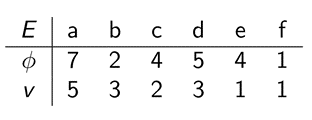
\includegraphics[width=6cm]{images/tab_KP.png}
    \caption{Dataset}
    \label{fig:tab_KP}
\end{figure}

\begin{figure}[H]
    \centering
    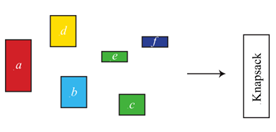
\includegraphics[width=6cm]{images/graphic_KP.png}
    \caption{Raffigurazione problema dello zaino}
    \label{fig:graphic_KP}
\end{figure}

\begin{figure}[H]
    \centering
    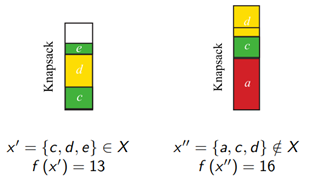
\includegraphics[width=8cm]{images/cand_sol_KP.png}
    \caption{Soluzioni candidate}
    \label{fig:cand_sol_KP}
\end{figure}

\begin{itemize}
    \item La prima soluzione candidata considera tre elementi la cui somma è $\leq V$, questo significa che la
          soluzione è un sottoinsieme preso dalla regione di fattibilità $X$ ed è una \textbf{soluzione fattibile}.
    \item La seconda soluzione candidata ha una somma di elementi pari a $10$, la quale è $>V$. Quindi questo sotto insieme
          non è appartenente alla regione di fattibilità $X$ (ma solo al ground set), perciò verrà chiamata \textbf{soluzione infattibile}.
\end{itemize}

Tra le soluzioni fattibili proposte la \textbf{funzione oggettiva} propone di prendere la soluzione \textit{massima}, ma visto che $x''$ non è fattibile, prenderemo come soluzione $x'$.
\subsubsection{Maximum Diversity Problem (MDP)}
Il problema della diversità massima, \textit{Maximum Diversity Problem}, è un problema importante per il corso e
verrà utilizzato come esempio per la parte di laboratorio. Questo è un problema
definito su uno spazio metrico, quindi uno spazio con la nozione di \textit{distanza}.

Dati:
\begin{itemize}
    \item Un insieme di punti $P$.
    \item Una funzione $d:P \times P \rightarrow \mathbb{N}$, la quale provvede la distanza tra le coppie di punti.
    \item Un numero $k\in {1,...,|P|}$, il quale è il numero di punti che si vuole selezionare.
\end{itemize}

Il problema chiede di selezionare da un insieme di punti $P$ un sottoinsieme di $k$ punti la cui sommatoria delle distanze tra le coppie dei punti sia massima.
Questo è un problema CO, perché il numero di sottoinsiemi possibili è finito, ed in particolare è un problema CO perché le soluzioni sono sottoinsiemi del ground set.
Il ground set, banalmente, è l'insieme dei punti $B\equiv P$, mentre la regione di fattibilità include tutti i sottoinsiemi composti da $k$ punti.
$$X=\left\{x\subseteq B : |x| = k \right\}$$
La funzione oggettiva è la sommatoria di tutte le distanze tra le coppie di punti in $x$:
$$max\underset{x\in X}{f(x)}=\sum_{(i,j):i,j\in x}d_{ij}$$

Per esempio, consideriamo un dataset costituito da $7$ punti e considerando un $k=3$, questo significa che vogliamo trovare
un sottoinsieme costituito da $3$ punti tale che le coppie abbiano distanza massima.

\begin{figure}[H]
    \centering
    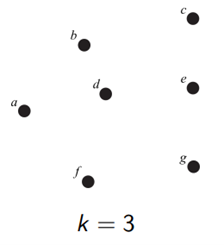
\includegraphics[width=3cm]{images/graph_MDP.png}
    \caption{Dataset}
    \label{fig:graph_MDP}
\end{figure}

\begin{figure}[H]
    \centering
    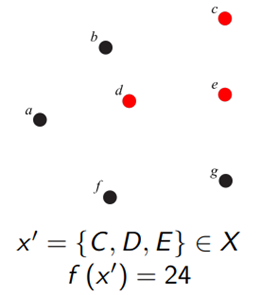
\includegraphics[width=3cm]{images/sol1_MDP.png}
    \caption{Prima soluzione candidata del MDP}
    \label{fig:cand_sol_MDP}
\end{figure}

\begin{figure}[H]
    \centering
    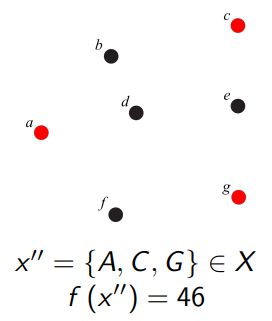
\includegraphics[width=3cm]{images/sol_MDP.png}
    \caption{Seconda soluzione candidata del MDP}
    \label{fig:cand_sol_2_MDP}
\end{figure}

La prima soluzione $x'$, considerando una metrica \textit{non fornita} ha come valutazione della funzione oggettiva $f(x')=24$, ed è un sottoinsieme tale per cui
la sua cardinalità sia $\leq k$, e quindi appartenente alla regione di fattibilità $X$.

La seconda soluzione ha come soluzione della funzione oggettiva $f(x'')=46$, questo è anche fattibile visto che $|x''|=k$, ed è una soluzione preferibile alla prima visto che
stiamo cercando il sottoinsieme che soddisfi massimo della funzione oggettiva.

\subsubsection{Interludio 1: la funzione oggettiva}
Fermiamoci un attimo e pensiamo qualcosa a riguardo di questo problema, in particolare soffermiamoci sulla funzione oggettiva.
Questa viene data come funzione che ha come dominio la regione di fattibilità e giunge al
codominio all'insieme dei numeri naturali.
$$f:X\rightarrow \mathbb{N}$$

Il calcolo di questa funzione potrebbe essere molto complesso ed estenuante, ogni singola soluzione ha il proprio valore rispetto alla funzione oggettiva
e si dovrebbe andare a controllare ogni volta in una tabella per svolgere il calcolo, non è una cosa molto interessante da fare.

Questo ovviamente, non è il caso dei precedenti problemi in quanto semplici da svolgere.

In particolare il problema KP una funzione oggettiva \textbf{additiva}, nel calcolare la $f$ dobbiamo effettuare delle somme
con il valore della funzione ausiliaria $\phi$ definita sul ground set, ricordando che nel problema KP, $B \equiv E$.
$$\phi : B\rightarrow \mathbb{N} \text{ induce } f(x)=\sum_{j\in x}\phi_j : X \rightarrow \mathbb{N}$$

Questo è interessante perché significa che si deve memorizzare solamente il valore della funzione
ausiliaria $\phi$, i quali sono $|B|$ valori, e non $2^B$, come sarebbe per i valori della funzione
oggettiva che è definita su $X$.
\newline
\newline
Lo stesso accade per il problema MDP e la sua funzione ausiliaria $d$, anche se quest'ultima ha una funzione oggettiva quadratica,
poi fornito un $n=|B|$ di punti nel caso peggiore si dovranno sommare $\frac{n(n-1)}{2}$ (numero di archi in un grafo completo) distanze, tuttavia però il
calcolo rimane \textit{"solamente"} una somma, quindi avente una \textbf{complessità polinomiale}.
\newline
Nel problema KP una volta che il valore viene fornito per uno specifico sottoinsieme, rimane possibile modificare gli elementi
e ricalcolare il valore della funzione oggettiva facilmente. Il valore della funzione oggettiva nel caso del MDP va trattato in maniera differente
per essere calcolato in tempo lineare (poiché quadratica).

Un'altra importante osservazione è che il problema KP e MDP sono definiti sull'intero insieme delle possibili (non fattibili)
soluzioni $2^B$, e questo è generalmente inutile visto che stiamo cercando
una soluzione fattibile (in alcuni casi questo però sarà utile).

Per riassumere, quando guardiamo un problema cerchiamo di capire come la funzione oggettiva è costituita:
\begin{itemize}
    \item È una funzione additiva?
    \item È una funzione quadratica?
    \item È una funzione semplice da calcolare?
    \item È una funzione semplice da aggiornare?
    \item Su cosa è definita la funzione oggettiva?
\end{itemize}

\subsection{Insieme dei problemi di partizionamento}
In questi problemi un insieme di oggetti viene fornito, l'obiettivo consiste nel dividerlo in sottoinsiemi ottenendo una partizione con alcune peculiarità.
\subsubsection{Bin Packing Problem (BPP)}
Il Bin Packing Problem (BPP), si ha un insieme di oggetti con un \textit{volume}, e si vuole mettere questi oggetti all'interno di
container con una \textit{capacità fissa} (fornita) utilizzando il \textbf{minimo numero di container}.

Dati:
\begin{itemize}
    \item Insieme $E$ di oggetti.
    \item Una funzione $v:E \rightarrow \mathbb{N}$ che fornisce il volume per un dato oggetto $e\in E$.
    \item Un insieme $C$ di containers.
    \item Un numero $V\in \mathbb{N}$ il quale rappresenta la capienza massima dei container (volume massimo contenibile).
\end{itemize}

La prima domanda che ci si vuole porre è: \textit{è un problema di ottimizzazione combinatoria?}

Il ground set è definito come $B=E\times C$, dove ogni elemento di $B$ è definito da una coppia $\langle oggetto, container\rangle$. Una soluzione
per questo problema è un sottoinsieme formato da oggetti di questo tipo, il prodotto cartesiano è necessario poiché si deve selezionare un oggetto ed inserirlo in un determinato container.

Una volta che la lista di coppie contenenti gli elementi di $E$
è costruita, una soluzione candidata sarà ottenuta (un sottoinsieme del ground set,
ma a noi questo non basta, voglia che sia un sottoinsieme della regione di fattibilità).
\newline
\newline
Consideriamo $B_e$ come il sottoinsieme del ground set dove gli oggetti delle coppie provengono da $E$ (i container sono tutti i possibili), e $B_c$ come il sottoinsieme del ground set dove i container nelle coppie degli elementi provengono da $C$ (gli elementi sono tutti i possibili).
$$B_e=\{(i,j) \in B : i=e\}$$
$$B_c=\{(i,j) \in B : i=c\}$$

La \textbf{regione di fattibilità} include tutte le partizione degli oggetti tra i
container tale per cui non ecceda la capacità di un qualsiasi container.
$$X=\left\{ x\subseteq B : |x\cap B_e|=1\text{ } \forall e \in E, \sum_{(e,c) \in B^c} v(e)\leq V \text{ } \forall c\in C \right\}$$

La prima parte dell'espressione è un vincolo sul sottoinsieme delle soluzioni fattibili $x$, dice che l'intersezione tra il sottoinsieme delle soluzioni fattibili ed il ground set deve avere modulo $1$. Questo significa che gli elementi
all'interno di $x$ devono essere presenti solamente una volta rispetto a gli elementi $E$ del ground set, ovvero $\in B_e$.

La seconda parte dell'espressione anch'essa è un vincolo ma rispetto al volume massimo dei container, dice che la somma dei volumi
di ogni singolo elemento del sottoinsieme fattibile non deve eccedere la capacità massima dei container $V$.

L'obiettivo è quello di minimizzare il numero di container utilizzati:
$$min\underset{x\in X}{f(x)}=|{c \in C : x\cap B^c \neq \emptyset}|$$

Per esempio, consideriamo degli oggetti con diversi volumi e sia data una capacità massima dei container pari a $V=4$.

\begin{figure}[H]
    \centering
    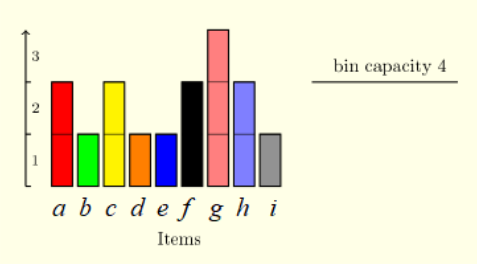
\includegraphics[width=6cm]{images/grap_BPP.png}
    \caption{Dataset}
    \label{fig:grap_BPP}
\end{figure}

\begin{figure}[H]
    \centering
    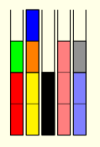
\includegraphics[width=2.5cm]{images/sol1_BPP.png}
    \caption{Prima soluzione candidata del Bin Packing Problem}
    \label{fig:sol1_BPP}
\end{figure}

Consideriamo la prima soluzione proposta, visto che la lista dei prodotti cartesiano
rispetta i due vincoli nella definizione della regione
di fattibilità la soluzione $x'$ è una \textbf{soluzione fattibile}.
$$x'=\left\{(a,1),(b,1),(c,2),(d,2),(e,2),(f,3),(g,4),(h,5),(i,5)\right\}\in X$$
$$f(x')=5$$

\begin{figure}[H]
    \centering
    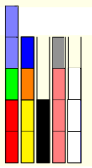
\includegraphics[width=2.5cm]{images/sol2_BPP.png}
    \caption{Seconda soluzione candidata del Bin Packing Problem}
    \label{fig:sol2_BPP}
\end{figure}

Invece, la seconda soluzione proposta è una \textbf{soluzione infattibile}, questo perché gli elementi non stanno
rispettando il secondo vincolo sul volume, e quindi
questo sottoinsieme non è compreso all'interno della regione di fattibilità.
$$x''=\left\{(a,1),(b,1),(c,2),(d,2),(e,2),(f,3),(g,4),(h,1),(i,4)\right\}\notin X$$
$$f(x'')=4$$
Considerando il caso in cui $x''$ fosse una soluzione fattibile avremmo scelto quella tra le soluzioni
proposte, poiché la funzione oggettiva effettua l'ottimizzazione sul minimo.

\subsubsection{Parallel Machine Scheduling Problem (PMSP)}
Il Parallel Machine Scheduling Problem (PMSP), è un problema nel quale un insieme di attività (tasks) deve essere diviso lungo un set di macchine in modo che
il \textit{tempo di completamento} sia minimizzato.

Dati:
\begin{itemize}
    \item Un insieme $T$ di tasks (o \textit{attività}).
    \item Una funzione $d:T \rightarrow \mathbb{N}$ che descrive la lunghezza (temporale) di ogni task.
    \item Un insieme di $M$ macchine.
\end{itemize}

Come prima, il ground set è dato dal prodotto cartesiano di due set forniti:
$$B\equiv T\times M$$
Significa che la soluzione deve essere una coppia $$\langle task,macchina\rangle$$. È importante
sottolineare che la sequenza in cui i task sono eseguiti non è rilevante, invece è rilevante il \textbf{tempo di completamento}
, ovvero il tempo con cui l'ultimo task termina (o il tempo in cui una macchina completa l'esecuzione dei suoi tasks).

La regione di fattibilità include tutte le partizioni delle attività nella macchine:
$$X=\left\{ x\subseteq B : |x\cap B_t|=1 \text{ } \forall t \in T \right\} $$
La \textbf{funzione oggettiva} ha come obiettivo quello di minimizzare il massimo della sommatoria delle lunghezze di tempo per ogni task di ogni macchina:
$$min\underset{x\in X}{f(x)}=max\underset{m\in M}{}\sum_{t:(t,m)\in x} d_t$$

In parole povere, vogliamo trovare il sottoinsieme $x$ che minimizza il tempo di completamento di ciascuna
macchina, dove il tempo di completamento per un singolo task è $\sum_{t:(t,m)\in x} d_t$.
\newline
\newline
Per esempio, consideriamo il seguente insieme di dati per tre macchine, $|M|=3$, e sette task differenti $|T|=7$.

\begin{figure}[H]
    \centering
    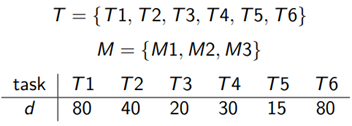
\includegraphics[width=5cm]{images/dataset_PMSP.png}
    \caption{Dataset del Parallel Machine Scheduling Problem}
    \label{fig:dataset_PMSP}
\end{figure}

\begin{figure}[H]
    \centering
    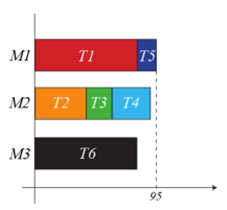
\includegraphics[width=4cm]{images/sol1_PMSP.png}
    \caption{Prima soluzione Parallel Machine Scheduling Problem}
    \label{fig:sol1_PMSP}
\end{figure}

Consideriamo la prima soluzione proposta:
$$x'=\left\{(T1,M1),(T2,M2),(T3,M2),(T4,M2),(T5,M1),(T6,M3)\right\}\in X$$
$$f(x')=95$$
Possiamo notare che questa è una \textbf{soluzione fattibile},
visto che ogni task accade al meno ed al massimo una volta.
Notiamo che il valore assunto dalla funzione oggettiva è $95$, questo proprio
perché l'ultimo task ha un tempo di completamento pari a $95$.

\begin{figure}[H]
    \centering
    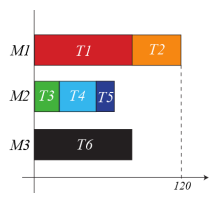
\includegraphics[width=4cm]{images/sol2_PMSP.png}
    \caption{Seconda soluzione Parallel Machine Scheduling Problem}
    \label{fig:sol2_PMSP}
\end{figure}

Consideriamo la seconda soluzione proposta:
$$x''=\left\{(T1,M1),(T2,M1),(T3,M2),(T4,M2),(T5,M2),(T6,M3)\right\}\in X$$
$$f(x'')=120$$
Notiamo che anche questa è una \textbf{soluzione fattibile} visto che ogni task accade al
minimo ed al massimo una volta, in questo casa la funzione oggettiva assume come valore $120$.
Questo significa che fra le due soluzioni proposte la prima è quella \textbf{ottima}.

\subsubsection{Interludio 2: la funzione oggettiva, ancora}
È necessario familiarizzare con il fatto che il ground set $B$ non è sempre uno degli insiemi
forniti nel problema, ma può essere formato dalla combinazione (come il prodotto cartesiano)
di diversi insiemi forniti. Ora affrontiamo la domande proposte nell'ultimo interludio.

\textit{Le funzioni oggettivi di che tipo sono? (additive, quadratiche,...)}
Questa volta le funzioni oggettive per il BPP e PMSP \textbf{non} sono additive, e non sono neanche banali.
È presente un algoritmo polinomiale per calcolare la funzione oggettiva, seppur non complesso,
non è semplice come per i problemi precedenti.

Notiamo che piccole modifiche alle soluzioni hanno un impatto \textit{variabile} sull'obiettivo, per esempio
consideriamo la seconda soluzione $x''$ del PMSP:
\begin{itemize}
    \item Spostare il task $T5$ sulla macchina $M1$, allunga il tempo di completamento complessivo$M1$,
          il risultato della funzione oggettiva cambia perché viene incrementato del task spostato (\textit{\textbf{impatto corrispondente al tempo del task spostato}}).
    \item Spostare il task $T5$ sulla macchina $M3$, non modifica il tempo di completamento complessivo
          delle macchine, il risultato della funzione oggettiva rimane lo stesso (\textit{\textbf{impatto zero}}).
    \item Spostare il task $T2$ sulla macchina $M2$, comporta una modifica dei tempi di completamento
          complessivi, il risultato della funzione oggettiva cambia poiché l'ultimo task viene spostato (\textit{\textbf{impatto intermedio}})

\end{itemize}

In fatti, l'impatto di una modifica di una soluzione dipende :
\begin{itemize}
    \item Da entrambi gli elementi modificati.
    \item E dagli elementi non modificati (questo è contrario alle cose dette nell'interludio 1).
\end{itemize}

Un punto interessante è che la funzione oggettiva del PMSP tende ad essere \textbf{piatta}, ovvero che sono presenti
molteplici soluzioni all'interno del problema dove il valore della funzione rimane lo stesso anche se avvengono
delle modifiche (l'esempio precedente, la soluzione $x''$ rimane fissa per diverse combinazioni su $120$).

\subsection{Problemi delle funzioni logiche}
\subsubsection{The Max-SAT problem}
Il problema del Max-Sat, sia da una formula in \textbf{forma normale congiuntiva}
(CNF, \textit{Conjunctive Normal Form}), si vogliono fornire in ingresso dei valori di
verità alle variabili logiche della CNF tali per cui la formula venga
soddisfatta (valutata come vera).

Dati:
\begin{itemize}
    \item Un insieme $V$ di \textbf{variabili logiche} $x_j$ con valori in $\mathbb{B}\in \{0,1\}$.
    \item Un \textbf{letterale} $l_j(x)\in {x_j,\overline{x}_j}$ che è una funzione che consiste in una variabile logica
          \textit{affermata} o \textit{negata}.
    \item Una \textbf{formula logica} $C_i(x)=l_{i,1} \lor ... \lor l_{i,n_i}$, la quale è
          una disgiunzione o \textit{somma logica} (OR) di letterali. Soddisfare una formula
          logica significa fargli assumere valore 1.
    \item Una formula in \textbf{forma normale congiuntiva} $CNF(x)=C_1\land ... \land C_n$ è una congiunzione di \textit{prodotti logici} di formule logiche.
    \item Una funzione $w$ che provvede dei \textit{pesi} per la formula CNF. La funzione associa ogni formula logica
          della CNF ad un rispettivo peso.
\end{itemize}

Visto che la soluzione consiste in un sottoinsieme caratterizzato dall'assegnamento
di valori di verità a variabili logiche, il \textbf{ground set} sarà il prodotto cartesiano
fra le variabili logiche e l'insieme dei numeri booleani:
$$B=V\times\mathbb{B}=\left\{(x_1,0),(x_1,1),...,(x_n,0),(x_n,1)\right\}$$

La \textbf{regione di fattibilità} è l'insieme delle soluzioni fattibili tali che una \textit{variabile}
venga considerata al più una volta. Essa include tutti sottoinsiemi costituenti
gli assegnamenti semplici che sono:
\begin{itemize}
    \item \textbf{completi}, ovvero che ad ogni variabile corrisponde \textit{almeno} un letterale.
    \item \textbf{consistenti}, ovvero che per ogni variabile corrisponde \textit{al massimo} un letterale.
\end{itemize}

$$X=\left\{x\subseteq B : |x\cap B_v|=1 \text{ }\forall v \in V \right\}$$
$$B_{xj}=\{(x_j,0),(x_j,1)\}$$

La \textbf{funzione oggettiva} (come sempre ottimizzata):
$$max\underset{x\in X}{f(x)}=\sum_{i:C_i(x)=1}w_i$$
L'obiettivo è quello di massimizzare il peso totale della \textit{formula logica soddisfatta}
segnata come $C_i(x)=1 \text{ per } i=1,...,n$ (dove $n$ è il numero di formule logiche presenti).

Consideriamo il seguente esempio:

$$V=\left\{x_1,x_2,x_3,x_4\right\}$$
$$L=\left\{x_1, \overline{x}_1, x_2, \overline{x}_3, x_3,\overline{x}_4, x_4\right\}$$
$$C_1=\overline{x}_1\lor x_2 \text{ ... } C_7=x_2$$
$$CNF = (\overline{x}_1\lor x_2 )\land (\overline{x}_1\lor x_3 )\land (\overline{x}_1\lor \overline{x}_3 )\land (\overline{x}_2\lor x_4 )\land (\overline{x}_2\lor \overline{x}_4 )\land x_1\land x_2$$
$$w_i=1 \forall C_i$$

Consideriamo adesso la seguente soluzione:
$$x=\left\{(x_1,0),(x_2,0),(x_3,1 ),(x_4,1)\right\}$$
La funzione oggettiva per questa soluzione assume valore $f(x)=5$, significa che soddisfa
$5$ formule delle $7$.

\textit{Risulta semplice trovare il valore della funzione oggettiva?} Non proprio, la complessità
della funzione oggettive è polinomiale

In caso di pesi uniformi sono presenti un campo ristretto di valori, che vanno da $0$ a $n$,
il numero di formule logiche, anche se sono presenti $2^|V|$ combinazioni che possono essere considerate.

\subsection{Problemi con matrici numeriche}
\subsubsection{Set covering problem (SCP)}
Data una \textbf{matrice binaria} ed una \textbf{funzione costo} definita per ogni
colonna della matrice (come vettore), si vuole selezionare il sottoinsieme di
colonne che coprono tutte le righe di costo minimo.

Dati:
\begin{itemize}
    \item Matrice binaria $A\in\mathbb{B}^{m,n}$ con insieme delle righe $R$ e insieme delle colonne $C$.
    \item La colonna $j\in C$ copre la riga $i\in R$ quando $a_{ij}=1$.
    \item Una funzione $c:C\rightarrow\mathbb{N}$ provvede il costo di ogni colonna.
\end{itemize}

Il \textbf{ground set} è l'insieme delle colonne.
$$B\equiv C$$
La \textbf{regione di fattibilità} include tutti i sottoinsiemi delle colonne che coprono
tutte le righe.
$$X=\left\{x\subseteq B : \sum_{j\in x}a_{ij}\geq 1 \text{ }\forall i \in R\right\}$$

L'obiettivo è \textit{minimizzare} il costo totale delle colonne selezionate, la \textbf{funzione oggettiva}
è additiva, molto veloce da calcolare ed aggiornare, però la \textit{fattibilità} non è
semplice da ottenere.
$$min\underset{x\in X}{f(x)}=\sum_{j\in x}c_j$$

Consideriamo il seguente esempio di una matrice con il relativo vettore dei costi:

\begin{figure}[H]
    \centering
    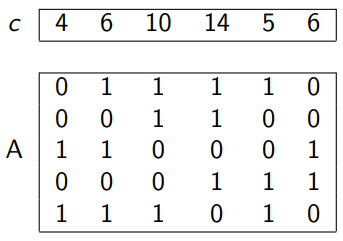
\includegraphics[width=5cm]{images/SCP_datasets.png}
    \caption{Dataset del Set Covering Problem (SCP)}
    \label{fig:dataset_SCP}
\end{figure}
Notiamo che la terza e la quinta riga (iniziando dall'alto) sono coperte dalla prima
colonna. Infatti, \textit{"set covering"}, si coprono i \textit{set} (righe) con
\textit{subset} (colonne).

Consideriamo adesso una prima soluzione proposta:
\begin{figure}[H]
    \centering
    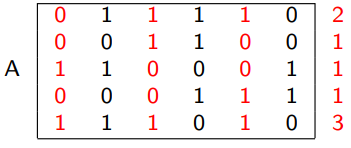
\includegraphics[width=5cm]{images/SCP_first_sol.png}
    \caption{Prima soluzione proposta del SCP}
    \label{fig:sol1_SCP}
\end{figure}

$$x'={c_1,c_2,c_5 }\in X$$
$$f(x')=19$$
La prima soluzione $x'$ è una \textbf{soluzione fattibile}, perché ogni riga ha almeno un elemento
$a_{ij}\geq 1$.

\begin{figure}[H]
    \centering
    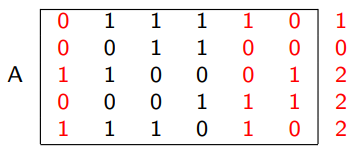
\includegraphics[width=5cm]{images/SCP_snd_sol.png}
    \caption{Seconda soluzione proposta del SCP}
    \label{fig:sol2_SCP}
\end{figure}

$$x''={c_1,c_5,c_6 }\notin X$$
$$f(x'')=15$$

La seconda soluzione $x''$ \textbf{non è una soluzione fattibile}, dato che la Seconda
riga non è coperta da almeno un elemento delle colonne. Comunque, nel caso in cui
la seconda soluzione sia una soluzione fattibile, allora quest'ultima sarebbe una
soluzione migliore della prima.

\subsubsection{Interludio 3: il test di fattibilità}
Solitamente, gli algoritmi euristici \textbf{richiedono} di risolvere il seguente
problema: \textit{Dato un sottoinsieme $x$, è fattibile o infattibile?}, in breve
$x\in X \text{?}$. Come risolvere questo problema? Innanzitutto, è un \textbf{problema di decisione}.

Consideriamo SCP, la fattibilità può essere decisa passando per ogni riga e sommando gli $1$ che appaiono
nella colonna selezionata: se una qualsiasi riga ha una somma complessiva pari a $0$ la soluzione sarà
\textbf{infattibile}.

Nel caso del KP, il test di fattibilità richiede di calcolare dalla soluzione e testare un singolo numero
(il peso totale rispetto alla capacità dello zaino) proprio come nel MDP, dove la cardinalità della soluzione
si trovava sotto una restrizione $k$.

Altri problemi come il Max-SAT ed il PMSP richiedono di testare la fattibilità su un singolo insieme di
numeri (numero di variabili logiche non si ripeta nella soluzione $x\cap B_v$), mentre problemi come il BPP richiedono di testare su diversi insiemi di numeri (i volumi degli oggetti rispetto
alla capacità dei container).

Alcune modifiche alle soluzioni vengono vietate \textit{a priori} per evitare l'inammissibilità delle soluzioni.
Supponiamo di avere una soluzione fattibile per il MDP, una qualsiasi modifica in cui il numero di punti non è uguale
al numero di punti aggiunti rende la soluzione \textbf{infattibile}.

Alcune modifiche non garantiscono \textbf{inammissibilità} (unfeasible) della soluzione, le quali richiedono un test
\textit{a posteriori} come nel PMSP.

\subsection{Set Packing Problem}
Il Set Packing Problem è un problema molto simile al precedente SCP, questo perché appartiene alla stessa
classe di problemi e provvede un valore per ogni colonna.


Dati:
\begin{itemize}
    \item Una \textbf{matrice binaria} $A\in \mathbb{B}^{m,n}$ con insieme delle righe $R$ e insieme delle colonne $C$.
    \item Sia definito un conflitto tra due colonne $j',j'' \in C$ quando $a_{ij'}=a_{ij''}=1$.
    \item Una funzione $\phi:C\rightarrow \mathbb{N}$ che provvede il valore di ogni colonna.
\end{itemize}
Il \textbf{ground set} è ancora l'insieme delle colonne:
$$B\equiv C$$
La \textbf{regione di fattibilità} include tutti i sottoinsieme di colonne che non sono in conflitto:
$$X=\left\{x\subseteq B:\sum_{j\in x}a_{ij}\leq 1 \text{ } \forall i \in R\right\}$$

L'obiettivo consiste nello scegliere le colonne di valore massimo senza che siano presenti \textit{conflitti}.
$$max\underset{x\in X}{f(x)}=\sum_{j \in x}\phi_j$$

Prendiamo in considerazione la seguente matrice:

\begin{figure}[H]
    \centering
    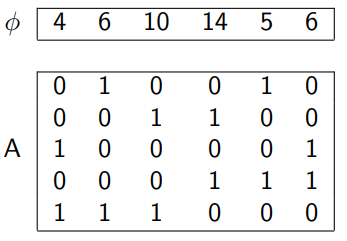
\includegraphics[width=5cm]{images/SPP_dataset.png}
    \caption{Dataset Set Packing Problem}
    \label{fig:datasets_SPP}
\end{figure}

\begin{figure}[H]
    \centering
    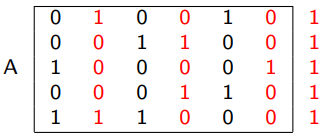
\includegraphics[width=5cm]{images/SPP_first_sol.png}
    \caption{Prima soluzione proposta del SPP (\textit{Set Packing Problem})}
    \label{fig:fst_sol_SPP}
\end{figure}


La prima soluzione proposta è $x'=\left\{c_2,c_4\right\}\in X$, con valutazione della funzione oggettiva
$f(x')=20$. Questa è una soluzione \textbf{fattibile}, visto che non presenti conflitti sulle righe delle colonne
selezionate.

\begin{figure}[H]
    \centering
    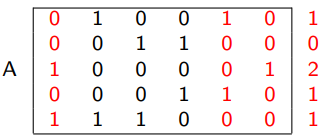
\includegraphics[width=5cm]{images/SPP_snd_sol.png}
    \caption{Seconda soluzione proposta del SPP (\textit{Set Packing Problem})}
    \label{fig:snd_sol_SPP}
\end{figure}
In questo caso \textbf{non è una soluzione fattibile}, visto che avviene il conflitto sulla terza riga, anche quando
la valutazione della funzione oggettiva era meglio della prima soluzione, le somme valutate non sono ottenute dalla
regione di fattibilità $X$.

\subsection{Set Partitioning Problem}
Il problema di Set Partitioning (non lo chiameremo con l'acronimo inglese), è una fusione dei due precedenti problemi
SCP e SPP.

Dati:
\begin{itemize}
    \item Una \textbf{matrice binaria} $A\in \mathbb{B}^{m,n}$ con insieme delle righe $R$ e insieme delle colonne
          $C$.
    \item Una funzione $c:C\rightarrow\mathbb{N}$ che fornisce il costo di ogni colonna.
\end{itemize}
La risoluzione del problema prevede di selezionare il sottoinsieme di \textit{costo minimo} delle colonne
che non sono in conflitto.
Il \textbf{ground set}, anche questa volta, è l'insieme delle colonne:
$$B\equiv C$$
La \textbf{regione di fattibilità} include tutti i sottoinsiemi di colonne che coprono tutte le righe che non
sono in conflitto:
$$X=\left\{x\subseteq C:\sum_{j\in x}a_{ij}=1 \text{ }\forall i \in R\right\}$$
$$min\underset{x\in X}{f(x)}=\sum_{j\in x}c_j$$

Consideriamo la seguente matrice binaria:

\begin{figure}[H]
    \centering
    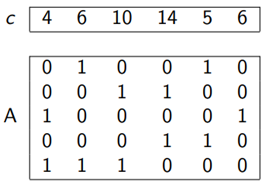
\includegraphics[width=5cm]{images/SPP2_dataset.png}
    \caption{Dataset del Set Partitioning Problem}
    \label{fig:dataset_SPP2}
\end{figure}

Ora prendiamo in considerazione la prima soluzione proposta:

\begin{figure}[H]
    \centering
    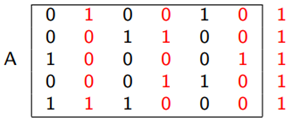
\includegraphics[width=5cm]{images/SPP2_fst_sol.png}
    \caption{Prima soluzione del SPP (\textit{Set Partitioning Problem})}
    \label{fig:fst_sol_SPP2}
\end{figure}

$$x'=\left\{c_2,c_3,c_6\right\}\in X$$
$$f(x')=26$$
Notiamo che la soluzione $x'$ è un \textbf{soluzione fattibile}, visto che gli elementi appartenenti alle
selezionati si trovano colonne si trovano in una maniera da non generare conflitti lungo le righe (la sommatoria
degli elementi lungo le righe non porta ad un risultato diverso da $1$).

Ora consideriamo la seconda soluzione candidata:
\begin{figure}[H]
    \centering
    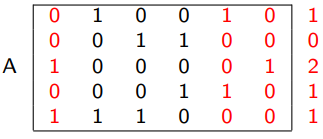
\includegraphics[width=5cm]{images/SPP2_snd_sol.png}
    \caption{Seconda soluzione del SPP (\textit{Set Partitioning Problem})}
    \label{fig:snd_sol_SPP2}
\end{figure}

$$x''=\left\{c_1,c_5,c_6\right\}\notin X$$
$$f(x'')=15$$

Anche se il risultato della funzione oggettiva ha un valore migliore (più piccolo) rispetto a quello della
prima soluzione, la soluzione $x''$ \textbf{non è una soluzione fattibile}. Questo perché, gli elementi sulla terza
riga si trovano in conflitto ($\sum_{j\in x}a_{ij}\geq 1$), ed anche perché la seconda riga non viene \textit{coperta}
da alcuna colonna ($\sum_{j\in x}a_{ij}=0$).

\subsection{Interludio 4: ricerca di soluzioni fattibili}
Gli algoritmi euristici spesso richiedono di risolvere un altro problema: \textit{trovare una soluzione
    che fattibile $x\in X$}, questo è un \textbf{problema di ricerca}. Chiaramente dato che le soluzioni
sono definite da una soluzione iniziale, le euristiche di scambio e ricombinazione hanno bisogno di
partire da un sottoinsieme valido tale per cui esso stesso sia una soluzione fattibile.

In base al problema la soluzione può essere banale:
\begin{itemize}
    \item Alcuni insiemi sono sempre fattibili: $x=\emptyset$ (come nel KP, SPP) o $x=B$ (nel SCP).
    \item Alcune soluzioni casuali soddisfano un vincolo come $|x|=k$ (nel MDP).
    \item Alcune soluzioni casuali soddisfano vincoli consistenti, come assegnare un task per ogni macchina
          come nel PMSP, o un valore ad ogni variabile logica come nel Max-SAT.
\end{itemize}
Oppure può essere difficile:
\begin{itemize}
    \item Nel BPP il numero di container deve essere sufficientemente grande.
    \item Nel SPP non è conosciuto alcun algoritmo polinomiale per risolvere il problema.
\end{itemize}

Alcuni algoritmi ingrandiscono al regione di fattibilità da $X$ a $X'$ (processo detto \textit{"rilassamento"}),
la funzione oggettiva $f$ deve essere estesa anch'essa da $X$ a $X'$, ma spesso $X'\setminus X$ provvede delle
soluzioni migliori.

\subsection{Problemi sui grafi}
\subsubsection{Vertex Cover Problem}
Dato un grafo indiretto $G=(V,E)$, selezionare un sottoinsieme di vertici di cardinalità minima tale che ogni
arco del grafo sia incidente a quest'ultimo.

Il \textbf{ground set} è l'insieme dei vertici:
$$B\equiv V$$
La \textbf{regione di fattibilità} include tutti i sottoinsiemi dei vertici tali che gli archi del grafo siano
incidenti ad essi:
$$X=\left\{x\subseteq V:x\cap (i,j)\neq\emptyset \text{ }\forall (i,j)\in E\right\}$$
L'obiettivo è minimizzare il numero di vertici selezionati:
$$min\underset{x\in X}{f(x)}=|x|$$

\begin{figure}[H]
    \centering
    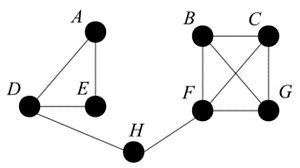
\includegraphics[width=5cm]{images/VCP_dataset.png}
    \caption{Dataset del Vertex Covering Problem}
    \label{fig:dataset_VCP}
\end{figure}

Prima soluzione proposta:
\begin{figure}[H]
    \centering
    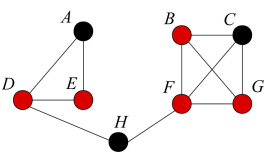
\includegraphics[width=5cm]{images/VCP_sol1.png}
    \caption{Prima soluzione proposta per il VCP}
    \label{fig:fst_sol_VCP}
\end{figure}

$$x'=\left\{ B,D,E,F,G \right\} \in X$$
$$f(x')=5$$
Notiamo che $x'$ è una \textbf{soluzione fattibile}, questo perché il sottoinsieme di vertici selezionato interseca
ogni arco del grafo (appartiene alla regione di fattibilità).

Guardiamo la seconda soluzione proposta:
\begin{figure}[H]
    \centering
    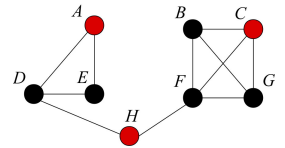
\includegraphics[width=5cm]{images/VCP_sol2.png}
    \caption{Seconda soluzione proposta per il VCP}
    \label{fig:snd_sol_VCP}
\end{figure}

Invece, la seconda soluzione \textbf{non è una soluzione fattibile}, anche se la funzione oggettiva porta ad un
risultato che è più convincente della soluzione precedente, questo sottoinsieme non appartiene alla regione di
fattibilità (il sottoinsieme di vertici selezionato non è incidente a tutti gli archi del grafo, e.g.: $(d,e)$).

\subsubsection{Maximum Clique Problem (MCP)}
Dati:
\begin{itemize}
    \item Un \textbf{grafo indiretto} $G=(V,E)$.
    \item Una funzione $w:V\rightarrow \mathbb{N}$ che provvede il peso di ogni vertice.
\end{itemize}
Selezionare il sottoinsieme di coppie di vertici adiacenti di peso massimo. Il \textbf{ground set} è l'insieme
dei vertici.
$$B\equiv V$$

La \textbf{regione di fattibilità} include tutti i sottoinsiemi di coppie di vertici adiacenti.
$$X=\left\{x\subseteq V:(i,v)\in E \text{ }\forall i \in x, \forall j \in x \setminus \{i\}\right\}$$
L'obiettivo è quello di massimizzare il peso dei vertici selezionati:
$$f(x)=\sum_{j\in x}w_j$$

Consideriamo il seguente grafo indiretto costituito da \textbf{pesi uniform} $w_i=1 \forall i\in V$.
\begin{figure}[H]
    \centering
    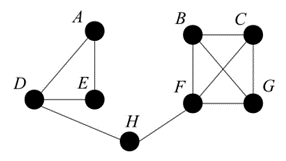
\includegraphics[width=5cm]{images/MCP_dataset.png}
    \caption{Dataset per il Maximum Clique Problem}
    \label{fig:MCP_dataset}
\end{figure}
Consideriamo la prima soluzione proposta:
\begin{figure}[H]
    \centering
    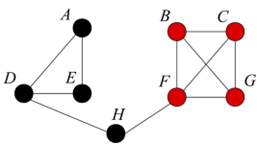
\includegraphics[width=5cm]{images/MCP_sol1.png}
    \caption{Prima soluzione proposta per il MCP}
    \label{fig:MCP_sol1}
\end{figure}
$$x'=\left\{B,C,F,G\right\}\in X$$
$$f(x')=4$$
La prima soluzione proposta è una soluzione \textbf{fattibile}, visto che ogni coppia nel sottoinsieme di vertici
presenta un arco tra di loro.
\begin{figure}[H]
    \centering
    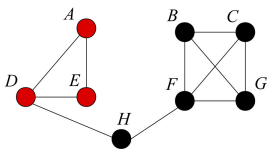
\includegraphics[width=5cm]{images/MCP_sol2.png}
    \caption{Seconda soluzione proposta per il MCP}
    \label{fig:MCP_sol2}
\end{figure}

$$x'=\left\{A,D,E\right\}\in X$$
$$f(x')=3$$
La seconda soluzione proposta è anch'essa una soluzione \textbf{fattibile}, per lo stesso motivo precedente.

\subsubsection{Maximum Independent Set}
Questo problema è opposto al MCP, vogliamo trvare un sottoinsieme di vertici di peso massimo che non è
connesso da archi.
Dati:
\begin{itemize}
    \item Un \textbf{grafo indiretto} $G=(V,E)$.
    \item Una funzione $w:V\rightarrow \mathbb{N}$ che provvede un peso per ogni arco.
\end{itemize}
Il \textbf{ground set} è l'insieme dei vertici.
$$B\equiv V$$
La \textbf{regione di fattibilità} include tutti i sottoinsiemi di vertici i cui archi \textit{non sono adiacenti}.
$$X=\left\{x\subseteq B : (i,j) \notin E \text{ }\forall i \in x, \forall j \in x\setminus \{i\}\right\}$$
L'obiettivo è quello di massimizzare il peso dei vertici selezionati.
$$max\underset{x\in X}{f(x)}=\sum_{j\in x}w_j$$
Consideriamo il seguente grafo indiretto con \textit{pesi uniformi}.
\begin{figure}[H]
    \centering
    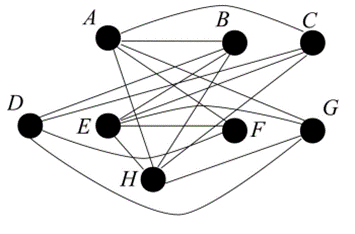
\includegraphics[width=5cm]{images/MIS_dataset.png}
    \caption{Dataset per il Maximum Independent Set}
    \label{fig:MIS_dataset}
\end{figure}
Adesso consideriamo la prima soluzione proposta:
\begin{figure}[H]
    \centering
    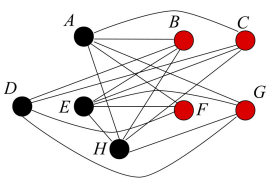
\includegraphics[width=5cm]{images/MIS_sol1.png}
    \caption{Prima soluzione per il MIS}
    \label{fig:MIS_1}
\end{figure}

$$x'=\left\{B,C,F,G\right\}\in X$$
$$f(x')=4$$
La soluzione $x'$ è una soluzione \textbf{fattibile}, ogni vertice del sottoinsieme proposto \textit{non è connesso}
con un altro vertice dello stesso sottoinsieme.

Consideriamo adesso una seconda proposta:
\begin{figure}[H]
    \centering
    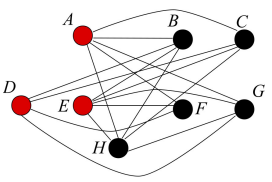
\includegraphics[width=5cm]{images/MIS_sol2.png}
    \caption{Seconda soluzione per il MIS}
    \label{fig:MIS_2}
\end{figure}

$$x''=\left\{A,D,E\right\}\in X$$
$$f(x'')=3$$
Anche la seconda soluzione è una \textbf{soluzione fattibile}.

\subsubsection{Interludio 5: le relazioni tra i problemi}
Come al solito le domande che uno si dovrebbe porre per un qualsiasi problema sono le solite :
\begin{itemize}
    \item \textit{Come si calcola la funzione oggettiva?}
    \item \textit{Cosa succede se togliamo un vertice?}
    \item \textit{Come si verifica la fattibilità?}
    \item \textit{Cosa succede se aggiungiamo o rimuoviamo un vertice ad una soluzione fattibile?}
\end{itemize}

Questi ultimi tre problemi sui grafi che abbiamo affrontato erano molto simili. Dovrebbe essere già noto
dalla \textbf{teoria delle complessità computazionali} che alcuni problemi possono essere \textbf{ridotti} ad altri
problemi, e che si possa \textit{utilizzare} un problema per risolverne un altro.

Un chiaro esempio è il seguente:
\begin{itemize}
    \item Si parte dall'istanza iniziale del MCP, con un grafo $G=(V,E)$.
    \item Si costruisce il \textbf{grafo complementare} $\overline{G}=(V,(V\times V)\setminus E)$ (un grafo tale
          per cui i vertici adiacenti nel grafo originario ora non lo sono più e viceversa).
    \item Si cerca una soluzione ottima per il MISP su $\overline{G}$.
    \item I vertici corrispondenti danno una soluzione ottimale del MCP su $G$.
\end{itemize}

\begin{figure}[H]
    \centering
    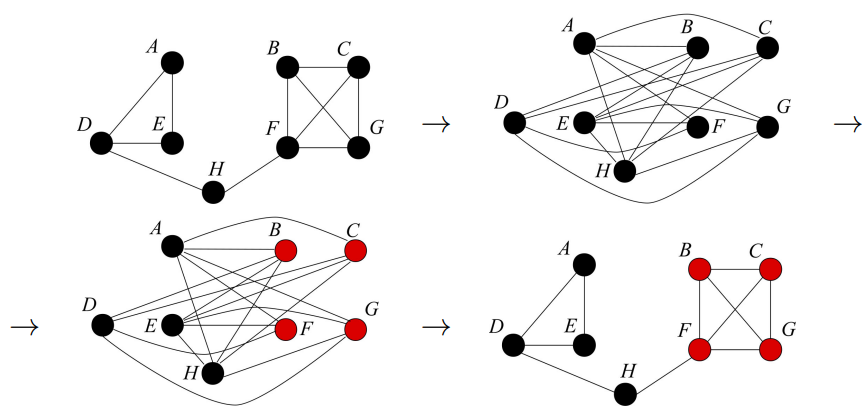
\includegraphics[width=10cm]{images/interlude5_complementary.png}
    \caption{Una soluzione euristica MISP che da una soluzione euristica MCP}
    \label{fig:interlude_5_graph}
\end{figure}

Questo processo può essere applicato anche nel verso opposto.

Anche i problemi SCP (\textit{Set Covering Problem}) e VCP (\textit{Vertex Covering Problem}) P hanno una relazione tra di loro, ma in maniera differente; ogni istanza del
VCP può essere trasformata in un istanza del SCP.
\begin{itemize}
    \item Ogni arco $i$ corrisponde ad una riga della matrice $A$.
    \item Ogni vertice $j$ corrisponde ad una colonna $A$.
    \item Se l'arco $i$ tocca il vertice $j$, l'insieme $a_{ij}=1$, altrimenti $a_{ij}=0$.
    \item Una soluzione ottimale del SCP da una soluzione ottimale del VCP.
\end{itemize}

\begin{figure}[H]
    \centering
    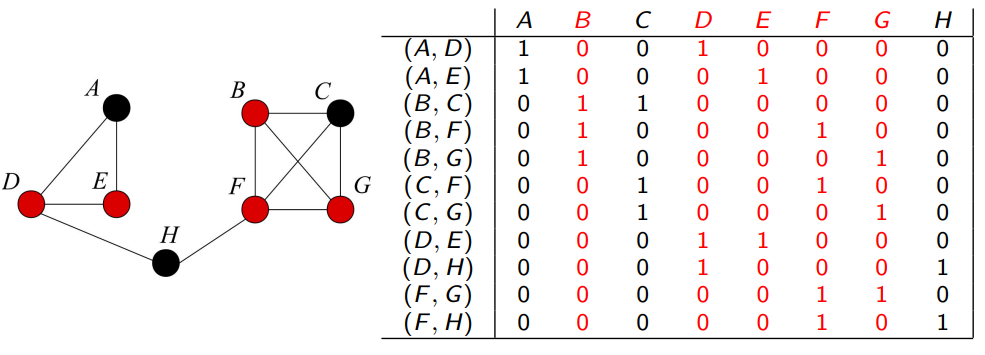
\includegraphics[width=10cm]{images/interlude5_vcp_scp.png}
    \caption{Una soluzione euristica SCP che da una soluzione euristica VCP}
    \label{fig:interlude5_vcp_scp}
\end{figure}
In questo caso non è semplice effettuare il procedimento inverso.

I problemi BPP (\textit{Bin Packing Problem}) e PMSP (\textit{Parallel Machine Scheduling Problem})
sono equivalenti, ma in una maniera più sofisticata:
\begin{itemize}
    \item I task corrispondono a gli oggetti.
    \item Le macchine corrispondono ai container, ma ricordiamo che il BPP cerca di ottimizzare il numero di
          container (data una capacità), mentre il PMSP dato un numero di macchine cerca di ottimizzare il \textit{tempo
              di completamento}.
\end{itemize}

Partiamo da un istanza del BPP:
\begin{itemize}
    \item Facciamo un assunzione sul numero di container ottimali, per esempio $3$.
    \item Costruiamo una corrispondente istanza nel PMSP.
    \item Calcoliamo il tempo di completamento ottimale, per esempio $95$; se eccede la capacità,
          incrementa l'assunzione fatta precedentemente (tipo $4$ o $5$). Nel caso contrario, decrementa
          l'assunzione fatta ($2$ o $1$).
\end{itemize}

\begin{figure}[H]
    \centering
    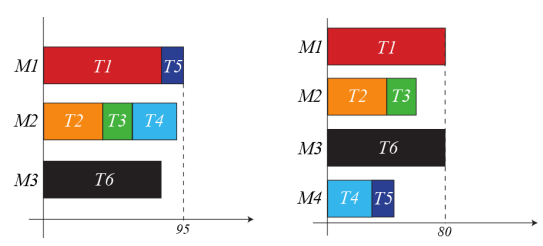
\includegraphics[width=10cm]{images/interlude5_BPP_scp.png}
    \caption{Una soluzione euristica PMSP che da una soluzione euristica BPP}
    \label{fig:interlude5_PMSP_BPP}
\end{figure}
Il processo inverso è possibile. I due problemi sono equivalenti, ma ognuno dei due deve venire risolto molteplici
volte.

È importante sottolineare il fatto che in caso di \textbf{riducibilità}, una soluzione euristica all'interno di un
istanza ridotta è una soluzione euristica per il problema originale; studiare le relazioni tra i problemi è importante
anche senza pensare agli algoritmi.

\subsubsection{Travelling Salesman Problem (TSP)}
Dato:
\begin{itemize}
    \item Un grafo \textbf{diretto} $G=(N,A)$
    \item Una funzione $c:A\rightarrow\mathbb{N}$ che provvede i costi per ogni arco.
\end{itemize}
Si vuole selezionare un ciclo di costo minimo che visiti tutti i nodi del grafo. Il \textbf{ground set} è l'insieme
degli archi.
$$B\equiv A$$
La \textbf{regione di fattibilità} include i cicli che visitano tutti i nodi del grafo (\textbf{cicli Hamiltoniani}).

L'obiettivo è minimizzare il costo totale degli archi selezionati.
$$min\underset{x\in X}{f(x)}=\sum_{j\in x}c_j$$

\textit{Come determinare quando un sottoinsieme è una soluzione fattibile?} Quel sottoinsieme deve identificare
un ciclo sul grafo ed ogni nodo deve avere esattamente un arco entrante ed uno uscente (ma sempre facente parte
del sottoinsieme). Inoltre, una visita del grafo utilizzando gli archi del sottoinsieme dovrebbe visitare tutti i
nodi, in altre parole non sono previste sotto visite di $G$.

\textit{Cosa accade se si effettua una modifica di una soluzione fattibile?} Questo dipende dal tipo della modifica
effettuata sulla soluzione, potrebbe essere necessario ricalcolare la funzione oggettiva.

\textit{Risulta difficile trovare una soluzione fattibile?} Trovare una soluzione che sia fattibile
potrebbe essere altrettanto difficile; in generale un grafo Hamiltoniano (ovvero che presenta un
ciclo Hamiltoniano) è un problema NP-completo, è di risoluzione banale solo nei grafi \textbf{completi}.

Consideriamo il seguente grafo diretto e pesato:
\begin{figure}[H]
    \centering
    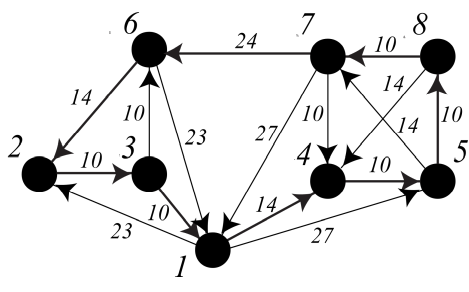
\includegraphics[width=7cm]{images/TSP_dataset.png}
    \caption{Dataset per il Travelling Salesman Problem}
    \label{fig:tsp_dataset}
\end{figure}

Consideriamo la prima soluzione proposta:
\begin{figure}[H]
    \centering
    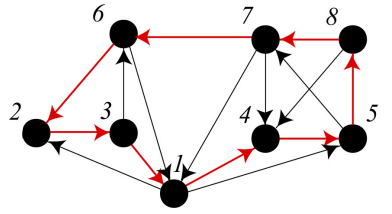
\includegraphics[width=7cm]{images/TSP_sol1.png}
    \caption{Prima soluzione del TSP}
    \label{fig:tsp_1_sol}
\end{figure}

$$x'=\left\{(1,4),(4,5),(5,8),(8,7),(7,6),(6,2),(2,3),(3,1)\right\}\in X$$
$$f(x')=102$$
La soluzione $x'$ è una soluzione \textbf{fattibile}.

Consideriamo la seconda soluzione proposta:
\begin{figure}[H]
    \centering
    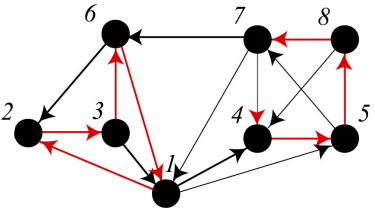
\includegraphics[width=7cm]{images/TSP_sol2.png}
    \caption{Seconda soluzione del TSP}
    \label{fig:tsp_2_sol}
\end{figure}
$$x''=\left\{(4,5),(5,8),(8,7),(7,4),(1,2),(2,3),(3,6),(6,1)\right\}\notin X$$
$$f(x'')=106$$
La soluzione $x''$ è una soluzione \textbf{fattibile}.

\subsubsection{Minimum Capacitated Spanning Tree Problem (MCSTP)}
Dati:
\begin{itemize}
    \item Un grafo indiretto $G=(V,E)$ con un vertice radice $r\in V$
    \item Una funzione $c:E\rightarrow \mathbb{N}$ che provvede il \textit{costo} di ogni arco.
    \item Una funzione $w:V\rightarrow \mathbb{N}$ che provvede il peso di ogni vertice.
    \item Un numero $W\in \mathbb{N}$ che è la capacità di ogni sotto albero.
\end{itemize}

Si vuole selezionare un \textbf{minimo albero ricoprente} tale che ogni ramo (sotto albero rispetto alla radice)
rispetti la capacità massima $W$. Il \textbf{ground set} è l'insieme degli archi.

$$B\equiv E$$

La \textbf{regione di fattibilità} include tutti gli alberi ricoprenti tali che il peso costituito dai vertici
rispetti la capacità $W$.
L'obiettivo è quello di minimizzare il costo totale degli archi selezionati.

$$min\underset{x\in X}{f(x)}=\sum_{j\in x}c_j$$

Consideriamo il seguente grafo indiretto di pesi uniformi $w_i=1 \forall i\in V$, e con una capacità massima
dei sotto alberi $W=3$.
\begin{figure}[H]
    \centering
    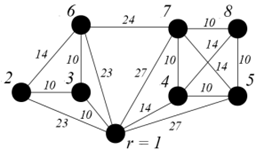
\includegraphics[width=5cm]{images/MCSTP_dataset.png}
    \caption{Dataset del Minimum Capacitated Spanning Tree Problem}
    \label{fig:dataset_MCSTP}
\end{figure}

La prima soluzione candidata:

\begin{figure}[H]
    \centering
    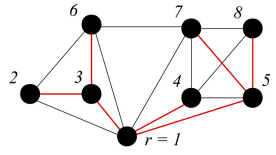
\includegraphics[width=5cm]{images/MCSTP_fst_sol.png}
    \caption{Prima soluzione del MCSTP}
    \label{fig:fst_sol_MCSTP}
\end{figure}

$$x'=\left\{(r,3),(3,2),(3,6),(r,4),(r,5),(5,7),(5,8)\right\}\in X$$
$$f(x')=95$$
Questa è una soluzione \textbf{fattibile}, visto che ogni sotto albero non eccede la
capacità $W$ e i sottoinsiemi sono un minimo albero ricoprente del grafo.

La seconda soluzione candidata:

\begin{figure}[H]
    \centering
    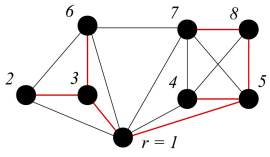
\includegraphics[width=5cm]{images/MCSTP_snd_sol.png}
    \caption{Seconda soluzione del MCSTP}
    \label{fig:snd_sol_MCSTP}
\end{figure}

$$x''=\left\{(r,3),(3,2),(3,6),(r,4),(r,5),(5,7),(5,8)\right\}\notin X$$
$$f(x'')=87$$
Questa \textbf{non è} una soluzione fattibile, visto che il sotto albero destro non rispetta
la capacità massima (nonostante il sottoinsieme sia un albero ricoprente).

Il costo delle operazioni principali cambia, il testi di fattibilità richeide solamente la somma
dei pesi, calcolare la funzione oggettiva richiede risolvere un problema
MST (\textit{Minimum Spanning Tree}).

La funzione oggettiva risulta:
\begin{itemize}
    \item \textbf{Lenta da valutare}, calcolare un MST per ogni sottoinsieme.
    \item \textbf{Lenta da aggiornare}, ricalcolare un MST per ogni sottoinsieme modificato.
\end{itemize}
Se il grafo è \textbf{completo}, i test di ammissibilità sono:
\begin{itemize}
    \item \textbf{Veloci da eseguire}, sommare i pesi dei vertici per ogni sotto albero.
    \item \textbf{Veloci da aggiornare}, sommare i pesi aggiunti e sottrarre quelli rimossi.
\end{itemize}
Visto che la funzione oggettiva è \textbf{additiva}, è abbastanza semplice da valutare, ma mentre
è semplice da ricalcolare, è più difficile verificarne la fattibilità, eccetto per situazioni banali.

Trovare uno \textbf{albero ricoprente capacitato} è un problema fortemente NP-completo, quindi spesso
è difficile trovare una soluzione fattibile a meno che il grafo sia completo. Dato un insieme di vertici,
in ordine si controlla se la soluzione è una soluzione fattibile o meno, è necessario costruire
la corretta rappresentazione dell'albero e poi visitare il sotto albero, sommare i pesi dei vertici, in
una maniera simile ad una visita DFS.
\newline
\newline
\textbf{Descrizione alternativa}
\newline


\subsubsection{Vehicle Routing Problem (VRP)}
\subsubsection{Interludio 6: combinare rappresentazioni alternative}
Il CMSTP ed il VRP condividono una complicazione interessante: differenti definizioni del
ground set $B$ sono possibili e naturali.
\begin{itemize}
    \item La descrizione come insieme di archi sembra preferibile per gestire la funzione oggettiva.
    \item La descrizione che utilizza un insieme di coppie $(vertice, albero)/(nodo/ciclo)$ sembra
          migliore per generare soluzioni ottime ed ha a che fare con la fattibilità.
\end{itemize}

\noindent\textit{Quale descrizione dovrebbe essere adottata?}
\newline\noindent Quella che rende più semplice le operazioni più frequenti, oppure una possibilità risulta
quella di utilizzare entrambe le rappresentazioni se le operazioni sono usate molto più frequentemente
che quanto sono aggiornate, in maniera che il fardello di mantenerle aggiornate e consistenti sia accettabile.

Per riassumere, le domande che ci si deve chiedere a riguardo di un problema sono:

\begin{itemize}
    \item Come si calcola la funzione oggettiva?
    \item Come provo che un sottoinsieme sia fattibile?
    \item Come trovo una soluzione fattibile?
    \item Come valutare il test di fattibilità?
    \item Cosa succede quando un cambiamento alla soluzione fattibile viene effettuato: è ancora fattibile?
          Sicuramente non lo è più? È necessario rivalutare da capo la funzione oggettiva o c'è una soluzione migliore?
    \item Quale è la definizione corretta di ground set? Sono qui presenti più definizioni possibili?
    \item Sono presenti relazioni tra questo ed un altro problema?
\end{itemize}

\section{Efficienza teorica}
La seconda parte di questo corso è dedicata alle caratteristiche degli algoritmi euristici: abbiamo precedentemente
descritto gli algoritmi euristici come algoritmi che non provvedono sempre soluzioni corrette, ma che sono
caratterizzati da due aspetti:
\begin{itemize}
    \item Costa molto meno degli algoritmi corretti.
    \item \textit{Spesso} restituisce qualcosa che è \textit{vicino} alla soluzione corretta.
\end{itemize}

Considereremo questi due aspetti, \textbf{costi} e \textbf{qualità}, significa la distanza e la probabilità
di ottenere una certa qualità e considereremo essi da due punti di vista:
\begin{itemize}
    \item \textit{Analisi a priori}, basata sulla teoria.
    \item \textit{Analisi a posteriori}, basata sull'evidenza e sui dati empirici ottenuti dall'esecuzione dell'algoritmo
          su dataset appositi per test.
\end{itemize}

\subsection{Problemi}
Informalmente, un problema è una domanda su un sistema costituito da oggetti matematici. La stessa domanda può
essere spesso posta su diversi sistemi simili.
\begin{itemize}
    \item Un istanza $I\in\mathcal{I}$ consiste in ogni specifico sistema riguardante la domanda.
    \item Una soluzione $S\in\mathcal{S}$ è una risposta corrispondente ad una delle istanze.
\end{itemize}

Per esempio: \textit{$n$ è un numero primo?}, questo è un problema con infinite istanze e due soluzioni.
$$\mathcal{I}=\mathbb{N}^+\setminus{\{1\}}\text{ and }\mathbb{S}=\text{\{yes,no\}}$$

Formalmente, un problema è una funzione che relaziona le istanze e le soluzioni:
$$P:\mathcal{I}\rightarrow\mathcal{S}$$
Definire una funzione non significa sapere come calcolarla.

\subsection{Algoritmi}
Un algoritmo è una \textbf{procedura formale}, composta da passi elementari posti in una sequenza finita, ogni
uno è determinato da un input e dai risultati dei passi precedenti.

Un algoritmo per un problema $P$ è un algoritmo tale per cui un input $I\in\mathcal{I}$ restituisce una soluzione
$S_I\in\mathcal{S}$.
$$A:\mathcal{I}\rightarrow\mathcal{S}$$
Un algoritmo definisce una funzione ed il modo per calcolarla, questo può essere:
\begin{itemize}
    \item \textbf{Esatto}, se la funzione associata coincide con il problema.
    \item Altrimenti \textbf{euristico}.
\end{itemize}
Un algoritmo euristico è utile se risulta:
\begin{itemize}
    \item \textbf{Efficiente}, significa che costa molto meno dell'algoritmo esatto.
    \item \textbf{Efficace}, significa che restituisce frequentemente la soluzione \textit{"vicina"} a quella corretta.
\end{itemize}

\subsection{Costi di un algoritmo euristico}
Il costo di un algoritmo (entrambi i tipi) denotano il costo di computazione durante esecuzione:

\begin{itemize}
    \item \textbf{Tempo}, richiesto per terminare la sequenza finita di passi elementari.
    \item \textbf{Spazio}, quello occupato in memoria dai risultati dei passi precedenti.
\end{itemize}

Il costo in tempo viene molto più discusso perché lo spazio è una risorsa rinnovabile, mentre il tempo non lo è.
Utilizzare lo spazio richiede di utilizzare meno tempo possibile, in oltre è tecnicamente più semplice distribuire
l'utilizzo di spazio che quello del tempo. Lo spazio ed il tempo sono parzialmente intercambiabili,
è possibile ridurre il costo di uno incrementando l'utilizzo dell'altro.

\subsubsection{Il tempo}
Il tempo richiesto per risolvere un problema dipende da diversi aspetti:
\begin{itemize}
    \item L'\textbf{istanza} specifica da risolvere.
    \item L'\textbf{algoritmo} utilizzato.
    \item La \textbf{macchina} che sta eseguendo l'algoritmo.
\end{itemize}
La nostra misura di tempo computazionale dovrebbe essere:
\begin{itemize}
    \item \textbf{Sconnessa} dalla tecnologia, che sia la stessa su macchine differenti.
    \item \textbf{Coincisa}, che viene riassunta in una semplice espressione simbolica.
    \item \textbf{Ordinale}, che sia sufficiente per essere comparata con diversi algoritmi.
\end{itemize}
Il tempo computazionale in secondo per ogni istanza viola tutti i requisiti.

\subsubsection{Complessità asintotica nel caso peggiore}
La complessità asintotica di un algoritmo nel \textbf{caso peggiore} provvede una tale misura
attraverso i seguenti passaggi:
\begin{enumerate}
    \item Definire il tempo come un numero $T$ di operazioni elementari eseguite.
    \item Definire la dimensione di un istanza come opportuno valore di $n$.
    \item Trovare il caso peggiore, ovvero il massimo valore di $T$ su tutte le istanze
          di dimensione $n$. $$T(n)=max\underset{I\in\mathcal{I}_n}{T(I)}\text{  ,  }n\in\mathbb{N}$$
          Ora la complessità in tempo è una funzione $T:\mathbb{N}\rightarrow\mathbb{N}$.
    \item Approssimare $T(n)$ da sotto e/o da sopra con una funzione più semplice $f(n)$, questo
          considerando solamente il loro comportamento asintotico (per $n\rightarrow\infty$).
    \item Collezionare le funzioni in \textbf{classi} con la stessa \textit{funzione di approssimazione}.
\end{enumerate}

\subsubsection{Gli spazi funzionali $\Theta$}
$$T(n) \in \Theta (f (n))$$
Formalmente significa:
$$\exists c_1, c_2 \in \mathbb{R}^+, n_0 \in \mathbb{N} : c_1 f(n) \leq T(n) \leq c_2 f(n)
    \text{  }\forall n\geq n_0$$

Dove $c_1,c_2$ e $n_0$ sono indipendenti da $n$. $T(n)$ è \textit{"racchiusa"} tra
$c_1 f(n)$ e $c_2 f(n)$, per:

\begin{itemize}
    \item Alcuni \textit{"piccoli"} valori di $c_1$.
    \item Alcuni \textit{"grandi"} valori di $c_2$.
    \item Alcuni \textit{"grandi"} valori di $n_0$.
\end{itemize}

\begin{figure}[H]
    \centering
    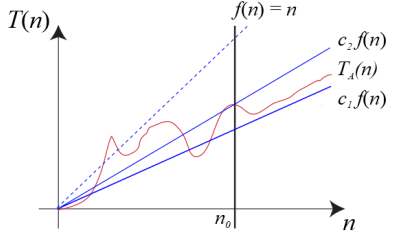
\includegraphics[scale=0.8]{images/theta.png}
    \caption{$f(n)=\Theta(T(n))$}
\end{figure}
Asintoticamente, la funzione $f(n)$ stima la funzione $T(n)$ per un fattore moltiplicativo:
per grandi istanze, il tempo computazionale è al meno ed al più il valore della funzione $f(n)$.

\subsubsection{Gli spazi funzionali $O$}
$$T (n) \in O (f (n))$$
Formalmente significa:
$$\exists c \in \mathbb{R}^+, n_0 \in \mathbb{N} : T(n) \leq c f(n) \text{  }\forall n \geq n_0$$

Dove $c$ e $n_0$ sono indipendenti da $n$. $T(n)$ è \textit{"dominata"} da $c f(n)$, per:
\begin{itemize}
    \item Alcuni \textit{"grandi"} valori di $c$.
    \item Alcuni \textit{"grandi"} valori di $n_0$.
\end{itemize}
Asintoticamente, la funzione $f(n)$ sovrastima la funzione $T(n)$ per un fattore moltiplicativo: per
grandi istanze, il tempo computazionale è al più proporzionale al valore della funzione $f(n)$
\begin{figure}[H]
    \centering
    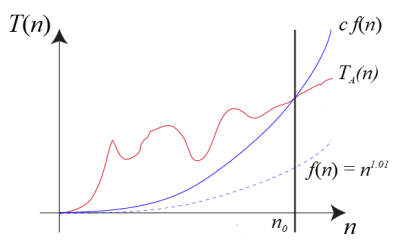
\includegraphics[scale=0.8]{images/ogrande.png}
    \caption{$f(n)=O(T(n))$}
\end{figure}

\subsubsection{Gli spazi funzionali $\Omega$}
$$T (n) \in \Omega (f (n))$$
Formalmente significa:
$$\exists c>0, n_0\in\mathbb{N}:T(n)\geq c f(n) \text{  }\forall n\geq n_0$$
Dove $c$ e $n_0$ sono indipendenti da $n$. $T(n)$ \textit{"domina"} $c f(n)$, per:
\begin{itemize}
    \item Alcuni \textit{"grandi"} valori di $c$.
    \item Alcuni \textit{"grandi"} valori di $n_0$.
\end{itemize}

\begin{figure}[H]
    \centering
    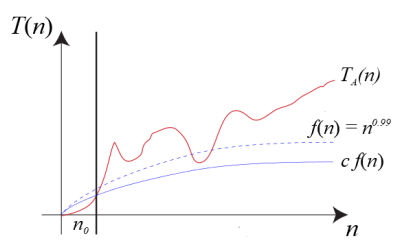
\includegraphics[scale=1]{images/omega.png}
    \caption{$f(n)=\Omega(T(n))$}
\end{figure}

Asintoticamente, $f(n)$ sovrastima $T(n)$ per un fattore moltiplicativo: per alcune grandi istanze,
il tempo computazionale è almeno proporzionale al valore della funzione $f(n)$.

\subsubsection{L'algoritmo esaustivo}
Per i problemi di ottimizzazione combinatoria la dimensione di un istanza può essere misurata
dalla cardinalità del ground set.
$$n=|B|$$

L'\textbf{algoritmo esaustivo}:
\begin{itemize}
    \item Considera ogni sottoinsieme $x\subseteq B$ tale che $x\in 2^{|B|}$.
    \item Testi la fattibilità (se $x\in X$) in un tempo $\alpha(n)$.
    \item In caso positivo, risolve la funzione oggettiva $f(x)$ in tempo $\beta(n)$.
    \item Se necessario, aggiorna il miglior valore trovato finora.
\end{itemize}

La complessità in tempo degli algoritmi esaustivi è :
$$T(n)\in\Theta\left( 2^n\left(\alpha(n)+\beta(n)\right) \right)$$
Questa risulta lo stesso esponenziale, anche se $\alpha(n)$ e $\beta(n)$ sono dei
polinomi (caso più frequente). La maggior parte delle volte l'algoritmo esaustivo
è \textbf{impraticabile}.

\subsubsection{Complessità polinomiale ed esponenziale}
Nei problemi di ottimizzazione combinatoria, la principale distinzione si trova tra:
\begin{itemize}
    \item \textbf{Complessità polinomiale}, $T(n)\in O(n^d)$, dove $d>0$ è costante.
    \item \textbf{Complessità esponenziale}, $T(n)\in\Omega(d^n)$, dove $d>1$ è costante.
\end{itemize}
Nella prima famiglia fanno parte gli \textbf{algoritmi efficienti}, invece nella seconda
quelli \textbf{inefficienti}. In generale, gli algoritmi euristici sono algoritmi polinomiali
per problemi dove l'algoritmo esatto risulta esponenziale.
\subsubsection{Problemi di trasformazione e riduzione}
Una relazione tra problemi permette la progettazione di algoritmi (\textit{interludio 5}).

Progettare un algoritmo per \textbf{trasformazione}:
\begin{enumerate}
    \item Data un istanza di un problema $P$, detta $I_P$, trasformarla in
          una istanza di un altro problema $Q$, $I_Q$.
    \item Data $I_Q$, applicare l'algoritmo $A_Q$ per ottenere la soluzione $S_Q$.
    \item Data $S_Q$, trasformiamola nella soluzione del problema $P$, $S_P$.
\end{enumerate}

Progettare un algoritmo per \textbf{riduzione}:
\begin{enumerate}
    \item Ripetere le trasformazioni $1,2,3$ diverse volte correggendo $I_Q$ basato sulle soluzioni
          $\{S_Q\}$ già ottenute.
\end{enumerate}

I due algoritmi spesso hanno complessità simili: se $A_Q$ è polinomiale (o esponenziale) e:
\begin{itemize}
    \item Costruire $I_Q$ impiegherà tempo polinomiale/esponenziale.
    \item Il numero di iterazioni sarà polinomiale/esponenziale.
    \item Costruire $S_P$ impiegherà tempo polinomiale/esponenziale.
\end{itemize}

Quindi $A_P$ è un algoritmo \textit{polinomiale/esponenziale}.

Il punto è che se si ha una trasformazione nella quale la modifica dell'istanza è
polinomiale, ed il tempo in cui la trasformazione è applicata è polinomiale, allora la
complessità di tutto l'algoritmo dipenderà dalla complessità di $A_Q$.

\subsubitem{Oltre alla complessità del caso peggiore}
La complessità nel caso peggiore ha diversi svantaggi:
\begin{itemize}
    \item Cancella tutte le informazioni delle istanze più semplici, poiché considera
          solamente le istanza con grandi dimensioni.

    \item Fornisce una approssimativa sovrastima del tempo computazionale, che
          in alcuni rari casi è inutile. Per esempio, i problemi di \textit{programmazione
              lineare}, nei quali i problemi hanno infinite soluzioni ma \textit{finite} soluzioni
          base, ed ammettono un algoritmo che ha complessità esponenziale.

          Tuttavia nella maggioranza dei casi gli algoritmi sono polinomi di bassa complessità.
\end{itemize}
\noindent\textit{Cosa se le istanze difficili sono rare nelle applicazioni pratiche?}
Per compensare, uno può investigare:
\begin{itemize}
    \item La \textbf{complessità parametrizzata}, la quale introduce un nuovo rilevante
          parametro $k$ (che è basato sulla dimensione di $n$), ed esprime il tempo come $T(n,k)$.
    \item La \textbf{complessità nel caso medio}, la quale si assume una probabilità di
          distribuzione su $\mathcal{I}$ ed esprime il tempo come il valore atteso.
          $$T(n)=E[T(I)|I\in \mathcal{I}_n]$$

\end{itemize}

\subsubsection{Complessità parametrizzata}
L'idea è che alcuni algoritmi non sono esponenziali in $n$ ma sono esponenziali in un
altro parametro $k$ che è più piccolo di $n$.

Se entrambi $k$ e $n$ sono grandi, allora ovviamente l'algoritmo è inefficiente, ma se $k$
è piccolo, allora l'algoritmo sarà efficiente e possibilmente anche polinomiale.

Perciò:
\begin{itemize}
    \item Efficiente su istanze con $k$ piccolo.
    \item Inefficiente su istanze con $k$ grande.
\end{itemize}

\begin{figure}[H]
    \centering
    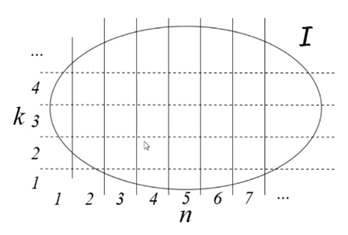
\includegraphics[scale=0.7]{images/param_coplx.png}
    \caption{Insieme delle istanza infinitamente diviso dai parametri $k$ ed $n$}
\end{figure}

Abbiamo tutti gli insiemi delle istanze del nostro problema, possiamo partizionare queste
istanze con un numero infinito di fette per $n$ e per l'altro parametro $k$. Possiamo
considerare il nostro algoritmo.

Il parametro $k$ può fare parte dell'input come la capacità, il massimo numero di
letterali per formula (SAT), il numero di elementi non-zero (problema matrici numeriche),
il massimo grado o il diametro (problemi con i grafi).

Stranamente il parametro aggiuntivo $k$ può essere parte della soluzione (come la \textit{
    cardinalità} nel VCP): in tale caso non puoi conoscere \textit{a priori} se l'algoritmo
è efficiente o meno, ma solo un approssimazione può essere disponibile. Quindi
se $k$ è facente parte della soluzione, solo \textit{a posteriori} sarà possibile
sapere se si tratta di un algoritmo efficiente.\newline

\subsubsection{Bounded tree search (algoritmo con parametro)}
\noindent\textbf{Per esempio: il VCP}
\newline
L'algoritmo esaustivo: per ogni uno dei $2^n$ sottoinsiemi di vertici, testare se
coprono tutti gli archi, calcolare la cardinalità e mantenere il valore più piccolo.
$$T(n,m)\in\Theta(2^n(m+n)),\text{ dove }n=|V|\text{ e }m=|E|$$

Ma se noi già sappiamo una soluzione con $f(x)=|x|=k+1$, possiamo cercare per una soluzione
di $k$ vertici, e progressivamente decrementare $k$ (o ancora meglio utilizzare
la \textbf{ricerca binaria} su $k$).

L'algoritmo naive: per ogni sotto insieme di $k$ vertici, testare se copre tutti gli archi.
$$T(n,m,k)\in\Theta(n^k m)$$
Per una dato $k$ fissato, l'algoritmo risulta di complessità polinomiale. Detto questo
è possibile fare di meglio.\newline\newline

\noindent\textbf{Bounded tree search per il VCP}
\newline
Un algoritmo migliore può essere basato sulla seguente proprietà:
$$x\cap(u,v)\neq\emptyset\text{ }\forall x\in X,(u,v)\in E$$
Ovvero, una qualsiasi soluzione fattibile include almeno un estremo (vertice)
di ogni arco.

Allora l'algoritmo \textbf{Bounded tree search} (\textit{ricerca delimitata da gli alberi}),
vuole trovare $x$ tale che $x\leq k$:
\begin{enumerate}
    \item Scegliere un qualsiasi arco $(u,v)$, sia che $u\in x$ che $u\notin x$ e
          che $v\in x$ (ovvero che uno degli estremi non faccia per forza parte dalla soluzione).
    \item Per ogni caso \textit{"aperto"}, rimuovere i vertici di $x$ e gli archi che
          essi coprono. $$V:=V\setminus x, E:=E\setminus\{e\in E:e\cap x\neq\emptyset\}$$
    \item Se $|x|\leq k$ e $E=\emptyset$, $x$ è la soluzione richiesta.
    \item Se $|x|=k$ e $E\neq\emptyset$, non è presente alcuna soluzione.
    \item Altrimenti ritorna al passo $1$.
\end{enumerate}
La complessità è $T(n,m,k)\in\Theta(2^km)$, polinomiale in $n$ ($m<n^2$). Per $n>>2$,
questo algoritmo è molto più efficiente di quello \textit{naive}.\newline
\noindent\textbf{Esempio del Bounded tree search}
\newline
Nel seguente grafo con $n=10,m=16$, \textit{è presente una soluzione con $|x|\leq 3$?} (quindi
$k=3$).
\begin{figure}[H]
    \centering
    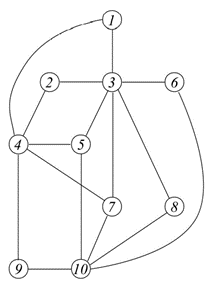
\includegraphics[scale=1]{images/bounded_tree_search_1.png}
    \caption{Stato iniziale del grafo (\textit{Bounded Tree Search})}
\end{figure}
\noindent Algoritmo esaustivo: $\Theta(2^n(m+n))$, con $2^n(m+n)=1024\cdot(16+10)$\newline
Algoritmo naive: $\Theta(n^k m)$, con $n^k m=1000\cdot 16$\newline
Bounded tree search algorithm: $\Theta(2^km)$ con $2^km=8\cdot 16$

\begin{figure}[H]
    \centering
    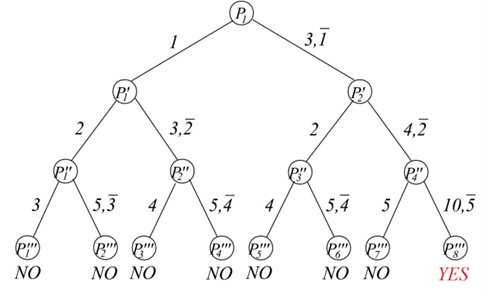
\includegraphics[scale=1]{images/bounded_tree_search_2.png}
    \caption{Soluzione del Bounded Tree Search, considerando un ordinamento lessicografico}
\end{figure}

\subsubsection{Kernelization - "Problem reduction" (algoritmo con parametro)}
La \textit{kernelizzazione} trasforma tutte le istanze di $P$ in istanze più
semplici di $P$, anziché istanze di un altro problema $Q$. Questa pratica è anche
conosciuta con il nome di \textbf{problem reduction} (\textit{riduzione del problema}).

Abbastanza spesso, in fatti, sono presenti delle proprietà molto utili che lo dimostrano:
\begin{itemize}
    \item Esiste una soluzione ottimale che non include certi elementi di $B$ (tali
          elementi possono essere rimossi).
    \item Esiste una soluzione ottimale che include certi elementi di $B$ (tali
          elementi possono essere messi da parte ed aggiunti dopo).
\end{itemize}
In breve rimuove elementi di $B$ senza modificare la soluzione. Possibili risultati
utili sono:
\begin{itemize}
    \item Un algoritmo esatto e polinomiale in $n$ (complessità parametrizzata).
    \item Algoritmi esatti più veloci ed algoritmi euristici.
    \item Migliori soluzioni euristiche.
    \item \textbf{Heuristic kernelization}, applica condizione rilassata sacrificando
          l'ottimalità.
\end{itemize}

\noindent Tornando al problema del VCP, vediamo la \textbf{Kernelization del VCP}:
\newline
Se $\delta_v\geq k+1$, il vertice $v$ appartiene ad una qualsiasi soluzione possibile di
valore $\leq k$. Considerare che $v$ ha $k+1$ archi incidenti e che dovrebbe essere
coperto da altrettanti vertici.
\newline
Algoritmo di kernelizzazione per mantenere solo i vertici della soluzione $x$ con $|x|\leq k$:
\begin{itemize}
    \item Iniziare allo step $t=0$ con $k_0=k$ ed un sottoinsieme di vertici vuoto $x_t:=\emptyset$
    \item Impostare $t=t+1$ ed aggiungere alla soluzione i vertici di grado $\geq k_t+1$.
          $$\delta_v\geq k_t+1\implies x_t := x_{t-1}\cup\{v\}$$
    \item Aggiornare $k_t\text{: } k_t:=k_0-|x_t|$
    \item Rimuovere i vertici con grado zero, quelli di $x$ e degli archi coperti.
          $$V:=\{v\in V : \delta_v > 0\}\setminus x_t$$
          $$E:=\{e\in E : e\cap x_t = \emptyset\}$$
    \item Se $|E|>k_t^2$, non è presente alcuna soluzione fattibile ($k_t$ vertici non sono abbastanza).
    \item Se $|E|\leq k_t^2\implies |V|\leq 2k_t^2$, si applica l'algoritmo esaustivo.
\end{itemize}
La complessità è $T(n,k)\in\Theta(n+m+2^{2k^2}k^2)$.

Per esempio, consideriamo il seguente grafo con $n=10,m=16$, \textit{è presente una
    soluzione con $|x|\leq k_0=5$?}
\begin{figure}[H]
    \centering
    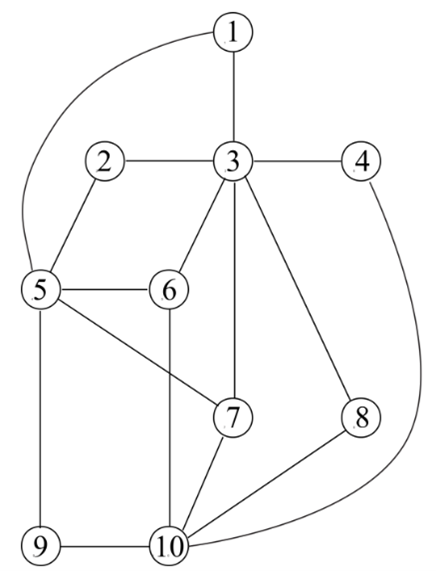
\includegraphics[scale=1]{images/kerneliz_0.png}
    \caption{Grafo d'esempio per la Kernelization del VCP}
\end{figure}

Algoritmo esaustivo:$\Theta(2^n(m+n))\implies T\approx 2^{10}(10+16)=26624$
\newline
\noindent Algoritmo naive: $\Theta(n^km)\implies T\approx 10^5\cdot 16=16000000$



\end{document}